% ==================================================================
%  §9.1  曲面的参数表示、切空间
%  源：徐森林、薛春华《数学分析》第二册，印刷页 135-157 (PDF p. 141-163)
%  底本：PaddleOCR-VL-1.6 JSON/MD 识别结果，人工逐字核校与公式精修
%  插图：原生 TikZ 逐幅复刻（图 9.1.1 ~ 图 9.1.9）
%  规范：全西文标点，忠实原文定义、注、定理、例题、练习题编号与推导
% ==================================================================

\section{曲面的参数表示、切空间}\label{sec:9.1}

\begin{definition}\label{def:9.1.1}
设 $\Delta$ 为 $\mathbb{R}^{s}$ 中的开集,
\[
  \boldsymbol{x}\colon \Delta \to \mathbb{R}^{n}, \quad \boldsymbol{u} = (u_{1}, u_{2}, \cdots, u_{s}) \mapsto \boldsymbol{x}(\boldsymbol{u}) = (x_{1}(u_{1}, u_{2}, \cdots, u_{s}), \cdots, x_{n}(u_{1}, u_{2}, \cdots, u_{s}))
\]
为映射, 则称 $M = \boldsymbol{x}(\Delta) = \{\boldsymbol{x}(\boldsymbol{u}) \mid \boldsymbol{u} \in \Delta\}$ 为 $s$ 维曲面, 而 $\boldsymbol{x}(\boldsymbol{u})$ 又称为 $M$ 的参数表示. 当 $\boldsymbol{x}(\boldsymbol{u})$ 为 $C^{k}\,(k \geqslant 0)$ 时, 称 $\boldsymbol{x}$ 或 $M$ 为 $C^{k}$ 曲面.
\end{definition}

如果 $\boldsymbol{x}$ 是 $C^{k}\,(k \geqslant 1)$ 的, 则称 $\boldsymbol{x}$ 或 $M$ 为 $s$ 维 $C^{k}$ 光滑曲面. 当
\[
  \operatorname{rank}(\boldsymbol{x}_{u_{1}}^{\prime}(\boldsymbol{u}^{0}), \boldsymbol{x}_{u_{2}}^{\prime}(\boldsymbol{u}^{0}), \cdots, \boldsymbol{x}_{u_{s}}^{\prime}(\boldsymbol{u}^{0}))
  = \operatorname{rank}\begin{pmatrix}
    \dfrac{\partial x_{1}}{\partial u_{1}} & \cdots & \dfrac{\partial x_{1}}{\partial u_{s}} \\
    \vdots & & \vdots \\
    \dfrac{\partial x_{n}}{\partial u_{1}} & \cdots & \dfrac{\partial x_{n}}{\partial u_{s}}
  \end{pmatrix}_{\boldsymbol{u}^{0}} = s
\]
时, 我们称 $\boldsymbol{u}^{0}$ 或 $\boldsymbol{x}(\boldsymbol{u}^{0})$ 为曲面或 $M$ 的正则点, 否则称为奇异点. 每个点都为正则点的曲面称为 $s$ 维 $C^{k}$ 正则曲面. 此时, $\{\boldsymbol{x}_{u_{1}}^{\prime}, \cdots, \boldsymbol{x}_{u_{s}}^{\prime}\}$ 处处是线性无关的.

当 $s = 1$ 时, 用 $t$ 表示参数, 一维曲面通常称为曲线, 考察一维 $C^{k}\,(k \geqslant 1)$ 曲线 $\boldsymbol{x}(t)$, 有(\cref{fig:9.1.1})
\begin{align*}
  \boldsymbol{x}^{\prime}(t) &= \lim_{\Delta t \to 0}\frac{\boldsymbol{x}(t + \Delta t) - \boldsymbol{x}(t)}{\Delta t} \\
  &= \left(\lim_{\Delta t \to 0}\frac{x_{1}(t + \Delta t) - x_{1}(t)}{\Delta t}, \lim_{\Delta t \to 0}\frac{x_{2}(t + \Delta t) - x_{2}(t)}{\Delta t}, \cdots, \lim_{\Delta t \to 0}\frac{x_{n}(t + \Delta t) - x_{n}(t)}{\Delta t}\right) \\
  &= (x_{1}^{\prime}(t), x_{2}^{\prime}(t), \cdots, x_{n}^{\prime}(t)),
\end{align*}
$t$ 为正则点等价于 $\operatorname{rank}\boldsymbol{x}'(t) = \operatorname{rank}(x'_1(t), x'_2(t), \cdots, x'_n(t)) = 1$; 等价于 $\boldsymbol{x}'(t) \neq \boldsymbol{0}$, 即 $x'_1(t), x'_2(t), \cdots, x'_n(t)$ 不全为 0.

\begin{figure}[htbp]
  \centering
  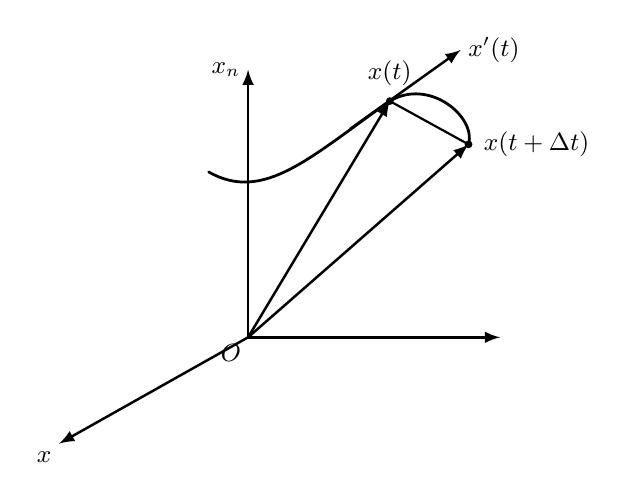
\begin{tikzpicture}[x=1.0cm, y=1.0cm, >=latex, line cap=round, line join=round]
    \draw[line width=0.9pt, ->] (0, 0) -- (-2.4, -1.35) node[below left=-1pt] {\small $x$};
    \draw[line width=0.9pt, ->] (0, 0) -- (3.2, 0);
    \draw[line width=0.9pt, ->] (0, 0) -- (0, 3.4) node[left=-1pt] {\small $x_n$};
    \node[below left=-1pt] at (0, 0) {\small $O$};

    \draw[line width=1.0pt] (-0.5, 2.1) .. controls (0.2, 1.7) and (0.8, 2.3) .. (1.8, 3.0)
                            .. controls (2.3, 3.3) and (2.9, 2.8) .. (2.8, 2.45);

    \coordinate (P) at (1.8, 3.0);
    \coordinate (Q) at (2.8, 2.45);

    \draw[line width=0.9pt, ->] (0, 0) -- (P);
    \draw[line width=0.9pt, ->] (0, 0) -- (Q);
    \draw[line width=0.8pt] (P) -- (Q);

    \draw[line width=0.9pt, ->] (1.3, 2.65) -- (2.7, 3.65) node[right=-1pt] {\small $\boldsymbol{x}'(t)$};

    \fill (P) circle (1.4pt) node[above=2pt] {\small $\boldsymbol{x}(t)$};
    \fill (Q) circle (1.4pt) node[right=2pt] {\small $\boldsymbol{x}(t + \Delta t)$};
  \end{tikzpicture}
  \caption{}\label{fig:9.1.1}
\end{figure}

我们称 $\boldsymbol{x}^{\prime}(t)$ 为曲线 $\boldsymbol{x}(t)$ 在 $t$ 点处的切向量. 当 $t$ 变动时, 得到一个沿曲线 $\boldsymbol{x}(t)$ 的切向量场. 如果 $\boldsymbol{x}(t)$ 为正则曲线, 则 $\dfrac{\boldsymbol{x}^{\prime}(t)}{\|\boldsymbol{x}^{\prime}(t)\|}$ 为沿曲线 $\boldsymbol{x}(t)$ 的单位切向量场. 应该强调的是 $\boldsymbol{x}^{\prime}(t)$ 或 $\dfrac{\boldsymbol{x}^{\prime}(t)}{\|\boldsymbol{x}^{\prime}(t)\|}$ 都是从 $\boldsymbol{x}(t)$ 点出发的向量.

\begin{definition}\label{def:9.1.2}
设 $\boldsymbol{x}(\boldsymbol{u})$ 为 $s$ 维 $C^{k}\,(k \geqslant 1)$ 正则曲面(也记为 $M$), 称 $\boldsymbol{x}'_{u_i}$ 为关于参数坐标 $u_{i}$ 的坐标切向量, 它是 $u_{i}$ 曲线(固定所有参数 $u_{j}\,(j \neq i)$, 只让 $u_{i}$ 变动时的曲线)的切向量. 由于 $\boldsymbol{x}(\boldsymbol{u})$ 为正则曲面, 故 $\operatorname{rank}(\boldsymbol{x}'_{u_1}, \boldsymbol{x}'_{u_2}, \cdots, \boldsymbol{x}'_{u_s}) = s$, 即 $\boldsymbol{x}'_{u_1}, \boldsymbol{x}'_{u_2}, \cdots, \boldsymbol{x}'_{u_s}$ 是线性无关的. 我们称由 $\{\boldsymbol{x}'_{u_1}(\boldsymbol{u}^0), \boldsymbol{x}'_{u_2}(\boldsymbol{u}^0), \cdots, \boldsymbol{x}'_{u_s}(\boldsymbol{u}^0)\}$ 张成的线性子空间
\[
  T_{\boldsymbol{x}(\boldsymbol{u}^{0})}M = \Big\{\sum_{i=1}^{s}\alpha_{i}\boldsymbol{x}_{u_{i}}^{\prime}(\boldsymbol{u}^{0}) \mathrel{\Big|} \alpha_{i} \in \mathbb{R}\Big\}
\]
为曲面 $M$(或 $\boldsymbol{x}(\boldsymbol{u})$)在点 $\boldsymbol{x}(\boldsymbol{u}^{0})$ 处的切空间. $T_{\boldsymbol{x}(\boldsymbol{u}^{0})}M$ 的每个向量称为曲面 $M$ 在点 $\boldsymbol{x}(\boldsymbol{u}^{0})$ 处的切向量. 显然, $T_{\boldsymbol{x}(\boldsymbol{u}^{0})}M$ 为 $s$ 维线性(向量)空间.
\end{definition}

\begin{theorem}\label{thm:9.1.1}
设 $\boldsymbol{x}(\boldsymbol{u})$ 在 $\boldsymbol{u}^{0} \in \Delta$ 处可微, 如果 $\{\boldsymbol{x}_{u_{1}}^{\prime}(\boldsymbol{u}^{0}), \boldsymbol{x}_{u_{2}}^{\prime}(\boldsymbol{u}^{0}), \cdots, \boldsymbol{x}_{u_{s}}^{\prime}(\boldsymbol{u}^{0})\}$ 线性无关, 即 $\operatorname{rank}\{\boldsymbol{x}_{u_{1}}^{\prime}(\boldsymbol{u}^{0}), \boldsymbol{x}_{u_{2}}^{\prime}(\boldsymbol{u}^{0}), \cdots, \boldsymbol{x}_{u_{s}}^{\prime}(\boldsymbol{u}^{0})\} = s$, $\boldsymbol{u}^{0} = \boldsymbol{u}(0)$ 为 $\boldsymbol{u}(t)$ 上一固定点, $\boldsymbol{u}(t)$ 在点 $0$ 处可导, 则
\[
  \frac{\mathrm{d}\boldsymbol{x}(\boldsymbol{u}(t))}{\mathrm{d}t}\bigg|_{t_0} \in T_{\boldsymbol{x}(\boldsymbol{u}^{0})}M,
\]
其中 $M = \boldsymbol{x}(\Delta)$(见\cref{def:9.1.1}).

反之, $\forall \boldsymbol{\alpha} \in \mathbb{R}^{s}$, $\sum_{i=1}^{s} \alpha_{i} \boldsymbol{x}_{u_{i}}^{\prime}(\boldsymbol{u}^{0}) \in T_{\boldsymbol{x}(\boldsymbol{u}^{0})}M$, 必 $\exists \boldsymbol{x}(\boldsymbol{u}(t)) \in M$, s.t. $\boldsymbol{u}(0) = \boldsymbol{u}^{0}$, 且
\[
  \frac{\mathrm{d}\boldsymbol{x}(\boldsymbol{u}(t))}{\mathrm{d}t}\bigg|_{t_0} = \sum_{i=1}^{s}\alpha_{i}\boldsymbol{x}_{u_{i}}^{\prime}(\boldsymbol{u}^{0}).
\]
这表明切空间 $T_{\boldsymbol{x}(\boldsymbol{u}^{0})}M$ 中的任一切向量都可用上述方式得到.
\end{theorem}

\begin{proof}
由于 $\boldsymbol{x}(\boldsymbol{u})$ 在 $\boldsymbol{u}^{0} = \boldsymbol{u}(0)$ 处可微, $\boldsymbol{u}(t)$ 在 $t = 0$ 处可导, 根据定理 8.2.2 与定理 8.2.6 知,
\[
  \frac{\mathrm{d}\boldsymbol{x}(\boldsymbol{u}(t))}{\mathrm{d}t}\bigg|_{t=0} = \sum_{i=1}^{s}\boldsymbol{x}_{u_{i}}^{\prime}(\boldsymbol{u}(0))u_{i}^{\prime}(0) = \sum_{i=1}^{s}u_{i}^{\prime}(0)\boldsymbol{x}_{u_{i}}^{\prime}(\boldsymbol{u}^{0}) \in T_{\boldsymbol{x}(\boldsymbol{u}^{0})}M.
\]
反之, $\forall \boldsymbol{\alpha} \in \mathbb{R}^s$, 令 $\boldsymbol{u}(t) = \boldsymbol{u}^0 + t\boldsymbol{\alpha}$, 则
\[
  \frac{\mathrm{d}\boldsymbol{x}(\boldsymbol{u}^{0} + t\boldsymbol{\alpha})}{\mathrm{d}t}\bigg|_{t=0} = \sum_{i=1}^{s}\alpha_{i}\boldsymbol{x}_{u_{i}}^{\prime}(\boldsymbol{u}^{0}) \in T_{\boldsymbol{x}(\boldsymbol{u}^{0})}M. \qedhere
\]
\end{proof}

曲面 $M$ 在点 $\boldsymbol{x}(\boldsymbol{u}^{0})$ 处的每个切向量 $\sum_{i=1}^{s}\alpha_{i}\boldsymbol{x}_{u_{i}}^{\prime}(\boldsymbol{u}^{0})$ 的起点都为 $\boldsymbol{x}(\boldsymbol{u}^{0})$, 其终点在 $\mathbb{R}^{n}$ 中可表示为(\cref{fig:9.1.2})
\[
  \boldsymbol{y} = \boldsymbol{x}(\boldsymbol{u}^{0}) + \sum_{i=1}^{s}\alpha_{i}\boldsymbol{x}_{u_{i}}^{\prime}(\boldsymbol{u}^{0}).
\]

\begin{figure}[htbp]
  \centering
  \begin{tikzpicture}[x=1.0cm, y=1.0cm, >=latex, line cap=round, line join=round]
    \draw[line width=0.9pt, ->] (0, 0) -- (-1.8, -1.2) node[below left=-1pt] {\small $x_1$};
    \draw[line width=0.9pt, ->] (0, 0) -- (4.0, 0) node[below=-1pt] {\small $x_2$};
    \draw[line width=0.9pt, ->] (0, 0) -- (0, 3.8) node[left=-1pt] {\small $x_3$};
    \node[below left=-1pt] at (0, 0) {\small $O$};

    \draw[line width=1.0pt] (0.8, 2.6) .. controls (1.5, 3.8) and (3.3, 3.6) .. (4.5, 2.8);
    \draw[line width=1.0pt] (0.8, 2.6) .. controls (1.2, 2.1) and (2.0, 2.4) .. (2.6, 2.0)
                            .. controls (3.2, 1.6) and (3.6, 0.9) .. (3.8, 1.0)
                            .. controls (4.0, 1.8) and (4.4, 2.1) .. (4.5, 2.8);
    \node at (4.0, 2.2) {\small $M$};

    \coordinate (X0) at (2.2, 2.6);

    \coordinate (PL1) at (1.8, 2.1);
    \coordinate (PL2) at (4.7, 2.4);
    \coordinate (PL3) at (4.9, 4.3);
    \coordinate (PL4) at (2.0, 4.0);
    \draw[line width=0.9pt] (PL1) -- (PL2) -- (PL3) -- (PL4) -- cycle;

    \draw[line width=0.7pt, dashed] (0, 0) -- ($(0,0)!0.65!(X0)$);
    \draw[line width=0.7pt] ($(0,0)!0.65!(X0)$) -- (X0);

    \draw[line width=1.0pt, ->] (X0) -- ++(1.4, 0.08) node[right=-1pt] {\small $\boldsymbol{x}'_{u_1}(\boldsymbol{u}^0)$};
    \draw[line width=1.0pt, ->] (X0) -- ++(0.15, 1.4) node[above=-1pt] {\small $\boldsymbol{x}'_{u_2}(\boldsymbol{u}^0)$};

    \coordinate (Y) at ($(X0) + (1.2, 1.1)$);
    \draw[line width=0.9pt, ->] (X0) -- (Y);
    \draw[line width=0.7pt, dashed] (0, 0) -- ($(0,0)!0.65!(Y)$);
    \draw[line width=0.7pt] ($(0,0)!0.65!(Y)$) -- (Y);

    \node[anchor=south west, inner sep=1pt] at (3.3, 3.4) {
      \small $\begin{aligned}
        &T_{\boldsymbol{x}(\boldsymbol{u}^0)}M \\
        &\boldsymbol{y} = \boldsymbol{x}(\boldsymbol{u}^0) + \sum_{i=1}^2 \alpha_i \boldsymbol{x}'_{u_i}(\boldsymbol{u}^0)
      \end{aligned}$
    };

    \fill (X0) circle (1.4pt) node[below=2pt] {\small $\boldsymbol{x}(\boldsymbol{u}^0)$};
  \end{tikzpicture}
  \caption{}\label{fig:9.1.2}
\end{figure}

\begin{example}\label{ex:9.1.1}
设 $\boldsymbol{x}\colon (a,b) \to \mathbb{R}^n$ 为 $C^k\,(k \geqslant 1)$ 正则曲线, 记为 $M$. $t_0 \in (a,b)$, 曲线 $\boldsymbol{x}(t)$ 在 $t_0$ 的切向量为 $\boldsymbol{x}'(t_0)$, 切空间 $T_{\boldsymbol{x}(t_0)} M = \{\alpha \boldsymbol{x}'(t_0) \mid \alpha \in \mathbb{R}\}$. 在 $\boldsymbol{x}(t_0)$ 处的切线为 $\boldsymbol{y} = \boldsymbol{x}(t_0) + \alpha \boldsymbol{x}'(t_0)$(向量形式), $\boldsymbol{x}(t_0)$ 为切线上的定点, $\boldsymbol{y}$ 为切线上的动点, $\alpha$ 为切线上的参数(\cref{fig:9.1.3}). 或坐标形式为
\[
  \frac{y_{1} - x_{1}(t_{0})}{x_{1}^{\prime}(t_{0})} = \frac{y_{2} - x_{2}(t_{0})}{x_{2}^{\prime}(t_{0})} = \cdots = \frac{y_{n} - x_{n}(t_{0})}{x_{n}^{\prime}(t_{0})} \, (=\alpha).
\]
\end{example}

\begin{figure}[htbp]
  \centering
  \begin{tikzpicture}[x=1.0cm, y=1.0cm, >=latex, line cap=round, line join=round]
    \draw[line width=0.9pt, ->] (0, 0) -- (-1.8, -1.2) node[below left=-1pt] {\small $x_1$};
    \draw[line width=0.9pt, ->] (0, 0) -- (3.8, 0) node[below=-1pt] {\small $x_2$};
    \draw[line width=0.9pt, ->] (0, 0) -- (0, 3.5) node[left=-1pt] {\small $y$};
    \node[below left=-1pt] at (0, 0) {\small $O$};

    \coordinate (X0) at (1.6, 2.3);

    \coordinate (N1) at (1.2, 3.5);
    \coordinate (N2) at (2.4, 2.7);
    \coordinate (N3) at (2.2, 0.4);
    \coordinate (N4) at (1.0, 1.2);
    \draw[line width=1.1pt] (N1) -- (N2) -- (N3) -- (N4) -- cycle;
    \node at (1.7, 1.4) {\small 法平面};

    \draw[line width=0.9pt] (0.5, 1.4) .. controls (1.1, 1.8) and (1.4, 2.2) .. (X0);
    \draw[line width=0.9pt] (X0) .. controls (1.9, 2.4) and (2.3, 2.7) .. (2.7, 2.6)
                            .. controls (3.1, 2.5) and (3.3, 2.1) .. (3.1, 1.6);
    \node[right=2pt] at (2.6, 2.1) {\small $\boldsymbol{x}(t)$};

    \draw[line width=0.8pt] (0.8, 1.7) -- ($(X0)!0.4!(0.8, 1.7)$);
    \draw[line width=0.8pt, dashed] ($(X0)!0.4!(0.8, 1.7)$) -- (X0);
    \draw[line width=0.8pt, dashed] (X0) -- ($(X0)!0.3!(3.0, 3.2)$);
    \draw[line width=0.9pt, ->] ($(X0)!0.3!(3.0, 3.2)$) -- (3.0, 3.2);
    \node[anchor=west] at (3.0, 3.2) {\small $\boldsymbol{y} = \boldsymbol{x}(t_0) + \alpha \boldsymbol{x}'(t_0)$};

    \draw[line width=0.8pt] (0.5, 2.6) -- (3.0, 1.2);
    \node[below right] at (2.7, 1.3) {\small 割线};

    \draw[line width=0.5pt, ->] (3.8, 3.7) node[right] {\small 切线} -- (3.05, 3.25);
    \draw[line width=0.5pt, ->] (2.2, 3.3) node[above] {\small 切方向} -- (X0);

    \fill (X0) circle (1.4pt) node[above left=-1pt] {\small $\boldsymbol{x}(t_0)$};
  \end{tikzpicture}
  \caption{}\label{fig:9.1.3}
\end{figure}

垂直切向量的超平面
\[
  x_{1}^{\prime}(t_{0})(y_{1} - x_{1}(t_{0})) + x_{2}^{\prime}(t_{0})(y_{2} - x_{2}(t_{0})) + \cdots + x_{n}^{\prime}(t_{0})(y_{n} - x_{n}(t_{0})) = 0
\]
称为曲线 $\boldsymbol{x}(t)$ 在 $\boldsymbol{x}(t_{0})$ 处的法平面. $\boldsymbol{x}(t_{0})$ 为法平面上的定点, 而 $\boldsymbol{y} = (y_{1}, y_{2}, \cdots, y_{n})$ 为法平面上的动点.

\begin{example}\label{ex:9.1.2}
设 $\Delta \subset \mathbb{R}^{2}$ 为开集, $\boldsymbol{x}\colon \Delta \to \mathbb{R}^{3}$, $(u, v) \mapsto \boldsymbol{x}(u, v) = (x(u, v), y(u, v), z(u, v))$ 为 $C^{k}\,(k \geqslant 1)$ 映射, $\operatorname{rank}(\boldsymbol{x}_{u}^{\prime}, \boldsymbol{x}_{v}^{\prime}) = 2$, $M = \boldsymbol{x}(\Delta)$ 为一个二维 $C^{k}$ 正则超曲面, 它的切空间为 $T_{\boldsymbol{x}(u,v)} M = \{\alpha_{1} \boldsymbol{x}_{u}^{\prime}(u, v) + \alpha_{2} \boldsymbol{x}_{v}^{\prime}(u, v) \mid \alpha_{1}, \alpha_{2} \in \mathbb{R}\}$.

在 $\boldsymbol{x}(u,v)$ 处的切超平面为(向量形式)
\[
  \boldsymbol{y} = \boldsymbol{x}(u,v) + \alpha_{1}\boldsymbol{x}_{u}^{\prime}(u,v) + \alpha_{2}\boldsymbol{x}_{v}^{\prime}(u,v).
\]
$\boldsymbol{x}(u,v)$ 为切超平面上的定点, $\boldsymbol{y}$ 为切超平面上的动点, $\alpha_{1}, \alpha_{2}$ 为切超平面上的参数.

与切超平面中从点 $\boldsymbol{x}(u,v)$ 出发的任何切向量 $\alpha_{1}\boldsymbol{x}'_{u}(u,v) + \alpha_{2}\boldsymbol{x}'_{v}(u,v)$ 都正交的向量称为 $\boldsymbol{x}(u,v)$ 点处的法向量. 显然, $\boldsymbol{n}$ 为法向量等价于 $\boldsymbol{n}$ 与 $\boldsymbol{x}'_{u}(u,v)$, $\boldsymbol{x}'_{v}(u,v)$ 都正交.

例如(\cref{fig:9.1.4}),
\begin{align*}
  \boldsymbol{n}(u,v) &= \boldsymbol{x}_{u}^{\prime}(u,v) \times \boldsymbol{x}_{v}^{\prime}(u,v) = \begin{vmatrix}
    \boldsymbol{i} & \boldsymbol{j} & \boldsymbol{k} \\
    \dfrac{\partial x}{\partial u} & \dfrac{\partial y}{\partial u} & \dfrac{\partial z}{\partial u} \\
    \dfrac{\partial x}{\partial v} & \dfrac{\partial y}{\partial v} & \dfrac{\partial z}{\partial v}
  \end{vmatrix} \\
  &= \frac{\partial(y,z)}{\partial(u,v)}\boldsymbol{i} + \frac{\partial(z,x)}{\partial(u,v)}\boldsymbol{j} + \frac{\partial(x,y)}{\partial(u,v)}\boldsymbol{k}
\end{align*}
或等于 $\left(\dfrac{\partial(y,z)}{\partial(u,v)}, \dfrac{\partial(z,x)}{\partial(u,v)}, \dfrac{\partial(x,y)}{\partial(u,v)}\right)$, 它既与 $\boldsymbol{x}_{u}^{\prime}(u,v)$ 正交, 又与 $\boldsymbol{x}_{v}^{\prime}(u,v)$ 正交. 因此, 上述的 $\boldsymbol{n}(u,v)$ 为超曲面 $M$ 在点 $\boldsymbol{x}(u,v)$ 处的法向量. 而切超平面的另一向量形式为
\[
  (\boldsymbol{y} - \boldsymbol{x}(u,v)) \cdot \boldsymbol{n}(u,v) = 0,
\]
其坐标形式为
\[
  \begin{vmatrix}
    y_{1} - x(u,v) & y_{2} - y(u,v) & y_{3} - z(u,v) \\
    \dfrac{\partial x}{\partial u} & \dfrac{\partial y}{\partial u} & \dfrac{\partial z}{\partial u} \\
    \dfrac{\partial x}{\partial v} & \dfrac{\partial y}{\partial v} & \dfrac{\partial z}{\partial v}
  \end{vmatrix} = 0.
\]
\end{example}

\begin{figure}[htbp]
  \centering
  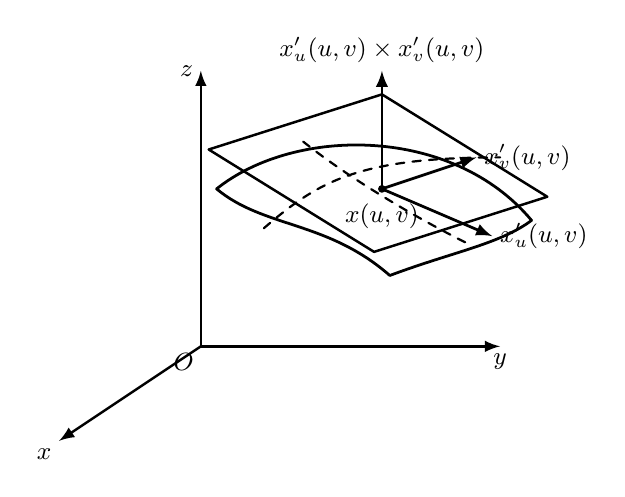
\begin{tikzpicture}[x=1.0cm, y=1.0cm, >=latex, line cap=round, line join=round]
    \draw[line width=0.9pt, ->] (0, 0) -- (-1.8, -1.2) node[below left=-1pt] {\small $x$};
    \draw[line width=0.9pt, ->] (0, 0) -- (3.8, 0) node[below=-1pt] {\small $y$};
    \draw[line width=0.9pt, ->] (0, 0) -- (0, 3.5) node[left=-1pt] {\small $z$};
    \node[below left=-1pt] at (0, 0) {\small $O$};

    \draw[line width=1.0pt] (0.2, 2.0) .. controls (1.2, 2.8) and (3.2, 2.8) .. (4.2, 1.6);
    \draw[line width=1.0pt] (0.2, 2.0) .. controls (0.8, 1.5) and (1.6, 1.6) .. (2.4, 0.9)
                            .. controls (3.2, 1.2) and (3.8, 1.3) .. (4.2, 1.6);

    \coordinate (XUV) at (2.3, 2.0);
    \draw[line width=0.8pt, dashed] (0.8, 1.5) .. controls (1.5, 2.1) and (2.0, 2.4) .. (3.8, 2.4);
    \draw[line width=0.8pt, dashed] (1.3, 2.6) .. controls (1.8, 2.2) and (2.6, 1.7) .. (3.4, 1.3);

    \coordinate (TP1) at (0.1, 2.5);
    \coordinate (TP2) at (2.2, 1.2);
    \coordinate (TP3) at (4.4, 1.9);
    \coordinate (TP4) at (2.3, 3.2);
    \draw[line width=0.9pt] (TP1) -- (TP2) -- (TP3) -- (TP4) -- cycle;

    \draw[line width=1.0pt, ->] (XUV) -- ++(1.4, -0.6) node[right=-1pt] {\small $\boldsymbol{x}'_u(u,v)$};
    \draw[line width=1.0pt, ->] (XUV) -- ++(1.2, 0.4) node[right=-1pt] {\small $\boldsymbol{x}'_v(u,v)$};
    \draw[line width=1.0pt, ->] (XUV) -- ++(0, 1.5) node[above=-1pt] {\small $\boldsymbol{x}'_u(u,v) \times \boldsymbol{x}'_v(u,v)$};

    \fill (XUV) circle (1.4pt) node[below=2pt] {\small $\boldsymbol{x}(u,v)$};
  \end{tikzpicture}
  \caption{}\label{fig:9.1.4}
\end{figure}

$\boldsymbol{n}(u,v)$ 通常不是单位向量. 现在, 我们来计算它的模. 由于
\begin{align*}
  \|\boldsymbol{x}_{u}^{\prime} \times \boldsymbol{x}_{v}^{\prime}\|^{2}
  &= (\|\boldsymbol{x}_{u}^{\prime}\| \|\boldsymbol{x}_{v}^{\prime}\| \sin\theta)^{2} \\
  &= \|\boldsymbol{x}_{u}^{\prime}\|^{2} \|\boldsymbol{x}_{v}^{\prime}\|^{2} (1 - \cos^{2}\theta) \\
  &= \|\boldsymbol{x}_{u}^{\prime}\|^{2} \|\boldsymbol{x}_{v}^{\prime}\|^{2} - (\boldsymbol{x}_{u}^{\prime} \cdot \boldsymbol{x}_{v}^{\prime})^{2} = EG - F^{2} = \det\begin{pmatrix} E & F \\ F & G \end{pmatrix},
\end{align*}
其中
\[
  \left\{\begin{aligned}
    E &= \boldsymbol{x}_{u}^{\prime} \cdot \boldsymbol{x}_{u}^{\prime} = \left(\frac{\partial x}{\partial u}\right)^{2} + \left(\frac{\partial y}{\partial u}\right)^{2} + \left(\frac{\partial z}{\partial u}\right)^{2}, \\
    F &= \boldsymbol{x}_{u}^{\prime} \cdot \boldsymbol{x}_{v}^{\prime} = \frac{\partial x}{\partial u}\frac{\partial x}{\partial v} + \frac{\partial y}{\partial u}\frac{\partial y}{\partial v} + \frac{\partial z}{\partial u}\frac{\partial z}{\partial v}, \\
    G &= \boldsymbol{x}_{v}^{\prime} \cdot \boldsymbol{x}_{v}^{\prime} = \left(\frac{\partial x}{\partial v}\right)^{2} + \left(\frac{\partial y}{\partial v}\right)^{2} + \left(\frac{\partial z}{\partial v}\right)^{2}.
  \end{aligned}\right.
\]
因此, $\boldsymbol{x}(u,v)$ 处的单位法向量为
\[
  \boldsymbol{n}_{0} = \pm\frac{\boldsymbol{x}_{u}^{\prime} \times \boldsymbol{x}_{v}^{\prime}}{\|\boldsymbol{x}_{u}^{\prime} \times \boldsymbol{x}_{v}^{\prime}\|} = \pm\frac{1}{\sqrt{EG - F^{2}}}\left(\frac{\partial(y,z)}{\partial(u,v)}, \frac{\partial(z,x)}{\partial(u,v)}, \frac{\partial(x,y)}{\partial(u,v)}\right).
\]
$E, F, G$ 称为曲面 $M$ 的第一基本量.

设参数 $(u,v)$ 与参数 $(\bar{u},\bar{v})$ 之间存在着一一对应的、一阶连续可导的对应关系
\[
  \left\{\begin{aligned}
    u &= u(\bar{u}, \bar{v}), \\
    v &= v(\bar{u}, \bar{v}),
  \end{aligned}\right. \quad (\bar{u}, \bar{v}) \in \bar{\Delta}, \; (u, v) \in \Delta.
\]
这时曲面 $M$ 有了新的参数表示:
\[
  \boldsymbol{x} = \boldsymbol{x}(u(\bar{u}, \bar{v}), v(\bar{u}, \bar{v})).
\]
直接的计算可知
\begin{align*}
  \bar{\boldsymbol{n}}(\bar{u}, \bar{v}) &= \boldsymbol{x}^{\prime}_{\bar{u}} \times \boldsymbol{x}^{\prime}_{\bar{v}} = \Big(\boldsymbol{x}^{\prime}_{u}\frac{\partial u}{\partial\bar{u}} + \boldsymbol{x}^{\prime}_{v}\frac{\partial v}{\partial\bar{u}}\Big) \times \Big(\boldsymbol{x}^{\prime}_{u}\frac{\partial u}{\partial\bar{v}} + \boldsymbol{x}^{\prime}_{v}\frac{\partial v}{\partial\bar{v}}\Big) \\
  &= \Big(\frac{\partial u}{\partial\bar{u}}\frac{\partial v}{\partial\bar{v}} - \frac{\partial u}{\partial\bar{v}}\frac{\partial v}{\partial\bar{u}}\Big)\boldsymbol{x}^{\prime}_{u} \times \boldsymbol{x}^{\prime}_{v} \\
  &= \frac{\partial(u,v)}{\partial(\bar{u},\bar{v})}\boldsymbol{x}^{\prime}_{u} \times \boldsymbol{x}^{\prime}_{v} = \frac{\partial(u,v)}{\partial(\bar{u},\bar{v})}\boldsymbol{n}(u,v).
\end{align*}
注意, 由于
\[
  1 = \frac{\partial(u,v)}{\partial(u,v)} = \frac{\partial(u,v)}{\partial(\bar{u},\bar{v})}\frac{\partial(\bar{u},\bar{v})}{\partial(u,v)},
\]
故
\[
  \frac{\partial(u,v)}{\partial(\bar{u},\bar{v})} \neq 0, \quad \frac{\partial(\bar{u},\bar{v})}{\partial(u,v)} \neq 0.
\]
如果 $\dfrac{\partial(u,v)}{\partial(\bar{u},\bar{v})} > 0\,(< 0)$, 则 $\bar{\boldsymbol{n}}(\bar{u},\bar{v})$ 与 $\boldsymbol{n}(u,v)$ 同(反)向, 我们称 $(\bar{u},\bar{v})$ 与 $(u,v)$ 为同(反)向的参数.

更一般地, 我们有下面结果.

\begin{example}\label{ex:9.1.3}
设 $\Delta \subset \mathbb{R}^{n-1}$ 为开集,
\[
  \boldsymbol{x}\colon \Delta \to \mathbb{R}^{n}, \quad \boldsymbol{u} = (u_{1}, u_{2}, \cdots, u_{n-1}) \mapsto \boldsymbol{x}(\boldsymbol{u}) = (x_{1}(\boldsymbol{u}), x_{2}(\boldsymbol{u}), \cdots, x_{n}(\boldsymbol{u}))
\]
为 $C^{k}\,(k \geqslant 1)$ 映射, $\operatorname{rank}(\boldsymbol{x}_{u_{1}}^{\prime}, \boldsymbol{x}_{u_{2}}^{\prime}, \cdots, \boldsymbol{x}_{u_{n-1}}^{\prime}) = n - 1$, $M = \boldsymbol{x}(\Delta)$ 为一个 $n - 1$ 维 $C^{k}$ 正则超曲面, 它的切空间为
\[
  T_{\boldsymbol{x}(\boldsymbol{u})}M = \Big\{\sum_{i=1}^{n-1}\alpha_{i}\boldsymbol{x}_{u_{i}}^{\prime}(\boldsymbol{u}) \mathrel{\Big|} \alpha_{i} \in \mathbb{R}, \, i = 1, 2, \cdots, n - 1\Big\}.
\]
在 $\boldsymbol{x}(\boldsymbol{u})$ 处的切超平面为(向量形式)
\[
  \boldsymbol{y} = \boldsymbol{x}(\boldsymbol{u}) + \sum_{i=1}^{n-1}\alpha_{i}\boldsymbol{x}_{u_{i}}^{\prime}(\boldsymbol{u}).
\]
$\boldsymbol{x}(\boldsymbol{u})$ 为切超平面上的定点, $\boldsymbol{y}$ 为切超平面上的动点, $\alpha_{1}, \alpha_{2}, \cdots, \alpha_{n-1}$ 为切超平面上的参数.

与切超平面中从点 $\boldsymbol{x}(\boldsymbol{u})$ 出发的任何切向量 $\sum_{i=1}^{n-1}\alpha_i \boldsymbol{x}'_{u_i}(\boldsymbol{u})$ 都正交的向量称为 $\boldsymbol{x}(\boldsymbol{u})$ 点处的法向量. 显然,
\[
  \boldsymbol{n} \text{ 为法向量} \iff \boldsymbol{n} \text{ 与每个 } \boldsymbol{x}'_{u_i}\,(i = 1, 2, \cdots, n - 1) \text{ 都正交}.
\]
例如, 设 $\{\boldsymbol{e}_{1}, \boldsymbol{e}_{2}, \cdots, \boldsymbol{e}_{n}\}$ 为 $\mathbb{R}^{n}$ 中的规范正交基(当 $n = 3$ 时, $\boldsymbol{e}_{1} = \boldsymbol{i}$, $\boldsymbol{e}_{2} = \boldsymbol{j}$, $\boldsymbol{e}_{3} = \boldsymbol{k}$), 则
\[
  \boldsymbol{n}(\boldsymbol{u}) = \begin{vmatrix}
    \boldsymbol{e}_{1} & \cdots & \boldsymbol{e}_{n} \\
    \dfrac{\partial x_{1}}{\partial u_{1}} & \cdots & \dfrac{\partial x_{n}}{\partial u_{1}} \\
    \vdots & & \vdots \\
    \dfrac{\partial x_{1}}{\partial u_{n-1}} & \cdots & \dfrac{\partial x_{n}}{\partial u_{n-1}}
  \end{vmatrix} = \sum_{i=1}^{n}(-1)^{1+i}\frac{\partial(x_{1}, x_{2}, \cdots, \hat{x}_{i}, \cdots, x_{n})}{\partial(u_{1}, u_{2}, \cdots, u_{n-1})}\boldsymbol{e}_{i}
\]
与每个 $\dfrac{\partial\boldsymbol{x}}{\partial u_{i}}$ 正交 $(i = 1, 2, \cdots, n - 1)$, 其中 $\hat{x}_{i}$ 表示删去 $x_{i}$. 换言之,
\[
  \boldsymbol{n}(\boldsymbol{u}) \cdot \frac{\partial\boldsymbol{x}}{\partial u_{i}} = \begin{vmatrix}
    \dfrac{\partial x_{1}}{\partial u_{i}} & \cdots & \dfrac{\partial x_{n}}{\partial u_{i}} \\
    \dfrac{\partial x_{1}}{\partial u_{1}} & \cdots & \dfrac{\partial x_{n}}{\partial u_{1}} \\
    \vdots & & \vdots \\
    \dfrac{\partial x_{1}}{\partial u_{n-1}} & \cdots & \dfrac{\partial x_{n}}{\partial u_{n-1}}
  \end{vmatrix} = 0.
\]
因此, 上述的 $\boldsymbol{n}(\boldsymbol{u})$ 为超曲面 $M$ 在点 $\boldsymbol{x}(\boldsymbol{u})$ 处的法向量, 而切超平面的另一向量形式为
\[
  (\boldsymbol{y} - \boldsymbol{x}(\boldsymbol{u})) \cdot \boldsymbol{n}(\boldsymbol{u}) = 0,
\]
其坐标形式为
\[
  \begin{vmatrix}
    y_{1} - x_{1}(\boldsymbol{u}) & \cdots & y_{n} - x_{n}(\boldsymbol{u}) \\
    \dfrac{\partial x_{1}}{\partial u_{1}} & \cdots & \dfrac{\partial x_{n}}{\partial u_{1}} \\
    \vdots & & \vdots \\
    \dfrac{\partial x_{1}}{\partial u_{n-1}} & \cdots & \dfrac{\partial x_{n}}{\partial u_{n-1}}
  \end{vmatrix} = 0.
\]
$\boldsymbol{n}(\boldsymbol{u})$ 通常不是单位向量. 当 $n \neq 3$ 时, 不能用 $\|\boldsymbol{x}'_{u} \times \boldsymbol{x}'_{v}\|$ 的方法来求 $\boldsymbol{n}(\boldsymbol{u})$ 的模. 但由其结果 $\|\boldsymbol{x}_{u}^{\prime} \times \boldsymbol{x}_{v}^{\prime}\|^{2} = \det\begin{pmatrix} E & F \\ F & G \end{pmatrix}$ 的启发, 我们有如下推导:

设 $g_{ij} = \boldsymbol{x}'_{u_i} \cdot \boldsymbol{x}'_{u_j} = \sum_{l=1}^{n} \dfrac{\partial x_l}{\partial u_i}\dfrac{\partial x_l}{\partial u_j}$, $i, j = 1, 2, \cdots, n - 1$. 则
\begin{align*}
  \|\boldsymbol{n}(\boldsymbol{u})\| &= \boldsymbol{n}(\boldsymbol{u}) \cdot \boldsymbol{n}_{0}(\boldsymbol{u}) = \begin{vmatrix}
    \boldsymbol{e}_{1} & \cdots & \boldsymbol{e}_{n} \\
    \dfrac{\partial x_{1}}{\partial u_{1}} & \cdots & \dfrac{\partial x_{n}}{\partial u_{1}} \\
    \vdots & & \vdots \\
    \dfrac{\partial x_{1}}{\partial u_{n-1}} & \cdots & \dfrac{\partial x_{n}}{\partial u_{n-1}}
  \end{vmatrix} \cdot \sum_{i=1}^{n}h_{i}\boldsymbol{e}_{i} \\
  &= \begin{vmatrix}
    h_{1} & \cdots & h_{n} \\
    \dfrac{\partial x_{1}}{\partial u_{1}} & \cdots & \dfrac{\partial x_{n}}{\partial u_{1}} \\
    \vdots & & \vdots \\
    \dfrac{\partial x_{1}}{\partial u_{n-1}} & \cdots & \dfrac{\partial x_{n}}{\partial u_{n-1}}
  \end{vmatrix} \\
  &= \sqrt{\det\begin{pmatrix}
    h_{1} & \cdots & h_{n} \\
    \dfrac{\partial x_{1}}{\partial u_{1}} & \cdots & \dfrac{\partial x_{n}}{\partial u_{1}} \\
    \vdots & & \vdots \\
    \dfrac{\partial x_{1}}{\partial u_{n-1}} & \cdots & \dfrac{\partial x_{n}}{\partial u_{n-1}}
  \end{pmatrix}\begin{pmatrix}
    h_{1} & \dfrac{\partial x_{1}}{\partial u_{1}} & \cdots & \dfrac{\partial x_{1}}{\partial u_{n-1}} \\
    \vdots & \vdots & & \vdots \\
    h_{n} & \dfrac{\partial x_{n}}{\partial u_{1}} & \cdots & \dfrac{\partial x_{n}}{\partial u_{n-1}}
  \end{pmatrix}} \\
  &= \sqrt{\det\begin{pmatrix}
    1 & 0 & \cdots & 0 \\
    0 & g_{11} & \cdots & g_{1,n-1} \\
    \vdots & \vdots & & \vdots \\
    0 & g_{n-1,1} & \cdots & g_{n-1,n-1}
  \end{pmatrix}} \\
  &= \sqrt{\det\begin{pmatrix}
    g_{11} & \cdots & g_{1,n-1} \\
    \vdots & & \vdots \\
    g_{n-1,1} & \cdots & g_{n-1,n-1}
  \end{pmatrix}} = \sqrt{\det(g_{ij})},
\end{align*}
其中 $\sum_{i=1}^{n}h_{i}\boldsymbol{e}_{i} = \boldsymbol{n}_{0}(\boldsymbol{u})$ 为与 $\boldsymbol{n}(\boldsymbol{u})$ 同方向的单位法向量. 因此, $\boldsymbol{x}(\boldsymbol{u})$ 处的单位法向量为
\[
  \boldsymbol{n}_{0}(\boldsymbol{u}) = \pm\frac{\boldsymbol{n}(\boldsymbol{u})}{\|\boldsymbol{n}(\boldsymbol{u})\|} = \pm\frac{1}{\sqrt{\det(g_{ij})}}\sum_{i=1}^{n}(-1)^{1+i}\frac{\partial(x_{1}, x_{2}, \cdots, \hat{x}_{i}, \cdots, x_{n})}{\partial(u_{1}, u_{2}, \cdots, u_{n-1})}\boldsymbol{e}_{i}.
\]
$g_{ij}\,(i, j = 1, 2, \cdots, n - 1)$ 称为超曲面 $M$ 的第一基本量. 当 $n = 3$ 时, $g_{11} = E$, $g_{12} = g_{21} = F$, $g_{22} = G$.

设参数 $(u_{1}, u_{2}, \cdots, u_{n-1})$ 与参数 $(\bar{u}_{1}, \bar{u}_{2}, \cdots, \bar{u}_{n-1})$ 之间存在着一一对应的、一阶连续可导的对应关系
\[
  \left\{\begin{aligned}
    u_{1} &= u_{1}(\bar{u}_{1}, \bar{u}_{2}, \cdots, \bar{u}_{n-1}), \\
    &\;\;\vdots \\
    u_{n-1} &= u_{n-1}(\bar{u}_{1}, \bar{u}_{2}, \cdots, \bar{u}_{n-1}),
  \end{aligned}\right. \quad \bar{\boldsymbol{u}} = (\bar{u}_{1}, \bar{u}_{2}, \cdots, \bar{u}_{n-1}) \in \bar{\Delta}, \; \boldsymbol{u} = (u_{1}, u_{2}, \cdots, u_{n-1}) \in \Delta.
\]
这时曲面 $M$ 有了新的参数表示:
\[
  \boldsymbol{x} = \boldsymbol{x}(\boldsymbol{u}(\bar{\boldsymbol{u}})) = \boldsymbol{x}(u_{1}(\bar{u}_{1}, \cdots, \bar{u}_{n-1}), u_{2}(\bar{u}_{1}, \cdots, \bar{u}_{n-1}), \cdots, u_{n-1}(\bar{u}_{1}, \cdots, \bar{u}_{n-1})).
\]
直接计算可知
\begin{align*}
  \bar{\boldsymbol{n}}(\bar{\boldsymbol{u}}) &= \begin{vmatrix}
    \boldsymbol{e}_{1} & \cdots & \boldsymbol{e}_{n} \\
    \dfrac{\partial x_{1}}{\partial\bar{u}_{1}} & \cdots & \dfrac{\partial x_{n}}{\partial\bar{u}_{1}} \\
    \vdots & & \vdots \\
    \dfrac{\partial x_{1}}{\partial\bar{u}_{n-1}} & \cdots & \dfrac{\partial x_{n}}{\partial\bar{u}_{n-1}}
  \end{vmatrix} = \sum_{i=1}^{n}(-1)^{1+i}\frac{\partial(x_{1}, x_{2}, \cdots, \hat{x}_{i}, \cdots, x_{n})}{\partial(\bar{u}_{1}, \bar{u}_{2}, \cdots, \bar{u}_{n-1})}\boldsymbol{e}_{i} \\
  &= \sum_{i=1}^{n}(-1)^{1+i}\frac{\partial(x_{1}, x_{2}, \cdots, \hat{x}_{i}, \cdots, x_{n})}{\partial(u_{1}, u_{2}, \cdots, u_{n-1})}\frac{\partial(u_{1}, u_{2}, \cdots, u_{n-1})}{\partial(\bar{u}_{1}, \bar{u}_{2}, \cdots, \bar{u}_{n-1})}\boldsymbol{e}_{i} \\
  &= \frac{\partial(u_{1}, u_{2}, \cdots, u_{n-1})}{\partial(\bar{u}_{1}, \bar{u}_{2}, \cdots, \bar{u}_{n-1})}\boldsymbol{n}(\boldsymbol{u}).
\end{align*}
\end{example}

注意, 由于
\[
  1 = \frac{\partial(u_{1}, u_{2}, \cdots, u_{n-1})}{\partial(u_{1}, u_{2}, \cdots, u_{n-1})} = \frac{\partial(u_{1}, u_{2}, \cdots, u_{n-1})}{\partial(\bar{u}_{1}, \bar{u}_{2}, \cdots, \bar{u}_{n-1})}\frac{\partial(\bar{u}_{1}, \bar{u}_{2}, \cdots, \bar{u}_{n-1})}{\partial(u_{1}, u_{2}, \cdots, u_{n-1})},
\]
故
\[
  \frac{\partial(u_{1}, u_{2}, \cdots, u_{n-1})}{\partial(\bar{u}_{1}, \bar{u}_{2}, \cdots, \bar{u}_{n-1})} \neq 0, \quad \frac{\partial(\bar{u}_{1}, \bar{u}_{2}, \cdots, \bar{u}_{n-1})}{\partial(u_{1}, u_{2}, \cdots, u_{n-1})} \neq 0.
\]
如果 $\dfrac{\partial(u_{1}, u_{2}, \cdots, u_{n-1})}{\partial(\bar{u}_{1}, \bar{u}_{2}, \cdots, \bar{u}_{n-1})} > 0\,(< 0)$, 则 $\bar{\boldsymbol{n}}(\bar{\boldsymbol{u}})$ 与 $\boldsymbol{n}(\boldsymbol{u})$ 同(反)向, 我们称 $(\bar{u}_{1}, \bar{u}_{2}, \cdots, \bar{u}_{n-1})$ 与 $(u_{1}, u_{2}, \cdots, u_{n-1})$ 为同(反)向的参数.

上面已详细讨论了 $C^{k}\,(k \geqslant 1)$ 正则超曲面的切空间, 法向量. 自然会问: $s$ 维 $C^{k}\,(k \geqslant 1)$ 的正则曲面的法空间应如何表示? 我们期望能用切空间 $T_{\boldsymbol{x}(\boldsymbol{u})}M$ 的基 $\{\boldsymbol{x}_{u_1}^{\prime}(\boldsymbol{u}),\allowbreak \boldsymbol{x}_{u_2}^{\prime}(\boldsymbol{u}),\allowbreak \cdots,\allowbreak \boldsymbol{x}_{u_s}^{\prime}(\boldsymbol{u})\}$ 来表达法空间
\[
  T_{\boldsymbol{x}(\boldsymbol{u})}^{\perp}M = \left\{\boldsymbol{n} \mathrel{\Big|} \boldsymbol{n} \perp T_{\boldsymbol{x}(\boldsymbol{u})}M, \text{ 即 } \boldsymbol{n} \cdot \boldsymbol{x}^{\prime}_{u_{i}}(\boldsymbol{u}) = 0, \, i = 1, 2, \cdots, s\right\},
\]
或者来表达法空间的一个基.

\begin{example}\label{ex:9.1.4}
设 $\boldsymbol{x}(\boldsymbol{u})$ 为 $s$ 维 $C^{k}\,(k \geqslant 1)$ 正则曲面, 则
\[
  (\boldsymbol{P} \quad \boldsymbol{Q}) = \begin{pmatrix}
    \dfrac{\partial\boldsymbol{x}(\boldsymbol{u})}{\partial u_{1}} \\
    \vdots \\
    \dfrac{\partial\boldsymbol{x}(\boldsymbol{u})}{\partial u_{s}}
  \end{pmatrix} = \begin{pmatrix}
    \dfrac{\partial x_{1}}{\partial u_{1}} & \cdots & \dfrac{\partial x_{n}}{\partial u_{1}} \\
    \vdots & & \vdots \\
    \dfrac{\partial x_{1}}{\partial u_{s}} & \cdots & \dfrac{\partial x_{n}}{\partial u_{s}}
  \end{pmatrix}.
\]
由于 $\operatorname{rank}(\boldsymbol{P} \quad \boldsymbol{Q}) = s$, 为叙述简单起见, 不妨设
\[
  \boldsymbol{P} = \begin{pmatrix}
    \dfrac{\partial x_{1}}{\partial u_{1}} & \cdots & \dfrac{\partial x_{s}}{\partial u_{1}} \\
    \vdots & & \vdots \\
    \dfrac{\partial x_{1}}{\partial u_{s}} & \cdots & \dfrac{\partial x_{s}}{\partial u_{s}}
  \end{pmatrix}
\]
为 $s \times s$ 非异矩阵. 因为
\begin{align*}
  (\boldsymbol{P} \quad \boldsymbol{Q})\left(-(\boldsymbol{P}^{-1}\boldsymbol{Q})^{\mathrm{T}} \quad \boldsymbol{I}_{n-s}\right)^{\mathrm{T}}
  &= (\boldsymbol{P} \quad \boldsymbol{Q})\begin{pmatrix} -\boldsymbol{P}^{-1}\boldsymbol{Q} \\ \boldsymbol{I}_{n-s} \end{pmatrix} \\
  &= -\boldsymbol{P}(\boldsymbol{P}^{-1}\boldsymbol{Q}) + \boldsymbol{Q}\boldsymbol{I}_{n-s} = -\boldsymbol{Q} + \boldsymbol{Q} = \boldsymbol{0},
\end{align*}
所以, $(\boldsymbol{P} \quad \boldsymbol{Q})$ 的行向量都正交于 $\left(-(\boldsymbol{P}^{-1}\boldsymbol{Q})^{\mathrm{T}} \quad \boldsymbol{I}_{n-s}\right)$ 的行向量. 此外, 显然有
\[
  \operatorname{rank}\left(-(\boldsymbol{P}^{-1}\boldsymbol{Q})^{\mathrm{T}} \quad \boldsymbol{I}_{n-s}\right) = n - s.
\]
因此, $\left(-(\boldsymbol{P}^{-1}\boldsymbol{Q})^{\mathrm{T}} \quad \boldsymbol{I}_{n-s}\right)$ 的 $n - s$ 个行向量为法空间 $T_{\boldsymbol{x}(\boldsymbol{u})}^{\perp}M$ 的一个基, 它由 $(\boldsymbol{P} \quad \boldsymbol{Q})$ 的元素所表达, 即由 $\dfrac{\partial x_{i}}{\partial u_{j}}\,(i = 1, 2, \cdots, n; \, j = 1, 2, \cdots, s)$ 所完全表达.
\end{example}

上述简洁的论述是难以想到的, 这是在查阅 Grassmann 流形 $G_{n-s,s}$ 与 $G_{s,n-s}$ 之间是微分同胚时, 见到的推导.

\begin{example}\label{ex:9.1.5}
设 $U \subset \mathbb{R}^n$ 为开集, $f\colon U \to \mathbb{R}^1$ 为 $C^k\,(1 \leqslant k \leqslant +\infty)$ 映射, 且在 $U$ 上,
\[
  \operatorname{rank} f = \operatorname{rank} \boldsymbol{J}f = \operatorname{rank}\left(\frac{\partial f}{\partial x_{1}}, \frac{\partial f}{\partial x_{2}}, \cdots, \frac{\partial f}{\partial x_{n}}\right) \equiv 1 \text{ (常值)},
\]
由例 8.4.5 知
\[
  M = f^{-1}(q) = \{\boldsymbol{x} \in U \mid f(\boldsymbol{x}) = q\} = \{\boldsymbol{x} \in U \mid f(\boldsymbol{x}) - q = 0\}
\]
{\emergencystretch=3em 或为空集, 或为 $n - 1$ 维 $C^{k}$ 流形或 $C^{k}$ 超曲面. 证明: 当 $M \neq \varnothing$ 时, $\operatorname{grad}f = \left(\dfrac{\partial f}{\partial x_{1}},\allowbreak \dfrac{\partial f}{\partial x_{2}},\allowbreak \cdots,\allowbreak \dfrac{\partial f}{\partial x_{n}}\right)$ 为 $M$ 的法向量场. 从而, 过定点 $\boldsymbol{x}^{0} \in M$ 的切超平面为\par}
\[
  (\boldsymbol{y} - \boldsymbol{x}^{0}) \cdot \operatorname{grad}f(\boldsymbol{x}^{0}) = 0,
\]
即
\[
  \sum_{i=1}^{n}\frac{\partial f}{\partial x_{i}}(\boldsymbol{x}^{0})(y_{i} - x_{i}^{0}) = 0.
\]
\end{example}

\begin{proof}[证法 1]
设 $M \neq \varnothing$, $\boldsymbol{x}(t)$ 为 $M$ 上过定点 $\boldsymbol{x}^{0} = \boldsymbol{x}(0)$ 的任一 $C^{1}$ 曲线, 则
\[
  f(\boldsymbol{x}(t)) \equiv q,
\]
两边对 $t$ 求导得到
\[
  \operatorname{grad}f \cdot \frac{\mathrm{d}\boldsymbol{x}}{\mathrm{d}t} = \sum_{i=1}^{n}\frac{\partial f}{\partial x_{i}}(\boldsymbol{x}(t))\frac{\mathrm{d}x_{i}}{\mathrm{d}t} \equiv 0,
\]
它表明 $f$ 的梯度向量 $\operatorname{grad}f \equiv \left(\dfrac{\partial f}{\partial x_{1}}, \dfrac{\partial f}{\partial x_{2}}, \cdots, \dfrac{\partial f}{\partial x_{n}}\right)\bigg|_{\boldsymbol{x}^{0}}$ 与曲面 $M$ 上点 $\boldsymbol{x}^{0}$ 处的切向量 $\boldsymbol{x}^{\prime}(0)$ 正交. 由于 $\boldsymbol{x}(t)$ 的任意性, $\operatorname{grad}f = \left(\dfrac{\partial f}{\partial x_{1}}, \dfrac{\partial f}{\partial x_{2}}, \cdots, \dfrac{\partial f}{\partial x_{n}}\right)\bigg|_{\boldsymbol{x}^{0}}$ 为 $T_{\boldsymbol{x}^{0}}M$ 的法向量.
\end{proof}

\begin{proof}[证法 2]
设 $M \neq \varnothing$, 不妨令 $\dfrac{\partial f}{\partial x_{n}} \neq 0$, 根据隐函数定理, 在局部, $x_{n} = x_{n}(x_{1}, x_{2}, \cdots, x_{n-1})$, 且
\[
  \frac{\partial x_{n}}{\partial x_{i}} = -\frac{\dfrac{\partial f}{\partial x_{i}}}{\dfrac{\partial f}{\partial x_{n}}}.
\]
由于局部参数表示为 $\boldsymbol{x} = \boldsymbol{x}(x_{1}, x_{2}, \cdots, x_{n-1}) = (x_{1}, x_{2}, \cdots, x_{n-1}, x_{n}(x_{1}, \cdots, x_{n-1}))$, 故
\[
  \left\{\begin{aligned}
    \boldsymbol{x}_{u_{1}}^{\prime} &= \left(1, 0, \cdots, 0, -\frac{\dfrac{\partial f}{\partial x_{1}}}{\dfrac{\partial f}{\partial x_{n}}}\right), \\
    &\;\;\vdots \\
    \boldsymbol{x}_{u_{n-1}}^{\prime} &= \left(0, 0, \cdots, 1, -\frac{\dfrac{\partial f}{\partial x_{n-1}}}{\dfrac{\partial f}{\partial x_{n}}}\right).
  \end{aligned}\right.
\]
显然,
\[
  \operatorname{grad}f \cdot \boldsymbol{x}_{u_{i}}^{\prime} = \left(\frac{\partial f}{\partial x_{1}}, \frac{\partial f}{\partial x_{2}}, \cdots, \frac{\partial f}{\partial x_{n}}\right) \cdot \left(0, \cdots, 0, \underset{\text{第 } i \text{ 个}}{1}, 0, \cdots, -\frac{\dfrac{\partial f}{\partial x_{i}}}{\dfrac{\partial f}{\partial x_{n}}}\right) = 0.
\]
因此, $\operatorname{grad}f = \left(\dfrac{\partial f}{\partial x_{1}}, \dfrac{\partial f}{\partial x_{2}}, \cdots, \dfrac{\partial f}{\partial x_{n}}\right)$ 为 $T_{\boldsymbol{x}(x_{1}, x_{2}, \cdots, x_{n-1})}M$ 的法向量. \qedhere
\end{proof}

\begin{definition}\label{def:9.1.3}
设 $\Delta_{i} \subset \mathbb{R}^{s_{i}}$ 为开集, $\varphi_{i}^{-1}\colon \Delta_{i} \to \varphi_{i}^{-1}(\Delta_{i}) \subset \mathbb{R}^{n_{i}}$ 为同胚, $i = 1, 2$, $\varphi_{1}^{-1}(\boldsymbol{u}) = \boldsymbol{x}(\boldsymbol{u})$ 为 $s_{1}$ 维 $C^{k}\,(k \geqslant 1)$ 正则曲面 $M_{1}$, $\varphi_{2}^{-1}(\boldsymbol{v}) = \boldsymbol{y}(\boldsymbol{v})$ 为 $s_{2}$ 维 $C^{k}$ 正则曲面 $M_{2}$. $\boldsymbol{u}(t)$ 为 $M_{1}$ 上的一条 $C^{1}$ 曲线. 如果映射 $f\colon M_{1} \to M_{2}$ 是 $C^{k}$ 的, 即 $\varphi_{2} \circ f \circ \varphi_{1}^{-1}\colon \Delta_{1} \to \Delta_{2}$ 为 $C^{k}$ 映射, 也就是分量
\[
  \left\{\begin{aligned}
    v_{1} &= (\varphi_{2} \circ f \circ \varphi_{1}^{-1})_{1}(u_{1}, u_{2}, \cdots, u_{s_{1}}), \\
    &\;\;\vdots \\
    v_{s_{2}} &= (\varphi_{2} \circ f \circ \varphi_{1}^{-1})_{s_{2}}(u_{1}, u_{2}, \cdots, u_{s_{1}})
  \end{aligned}\right.
\]
为 $C^{k}$ 的函数, 于是, $\boldsymbol{y} = \boldsymbol{y}(\boldsymbol{v}(\boldsymbol{u}(t))) = \boldsymbol{y}(\varphi_{2} \circ f \circ \varphi_{1}^{-1})(\boldsymbol{u}(t))$ 为 $M_{2}$ 上一条 $C^{1}$ 曲线. 易见,
\[
  f_{*}\left(\frac{\mathrm{d}\boldsymbol{x}}{\mathrm{d}t}\right) = \frac{\mathrm{d}\boldsymbol{y}}{\mathrm{d}t} = \sum_{j=1}^{s_{2}}\frac{\partial\boldsymbol{y}}{\partial v_{j}}\frac{\mathrm{d}v_{j}}{\mathrm{d}t} = \sum_{j=1}^{s_{2}}\frac{\partial\boldsymbol{y}}{\partial v_{j}}\sum_{i=1}^{s_{1}}\frac{\partial v_{j}}{\partial u_{i}}\frac{\mathrm{d}u_{i}}{\mathrm{d}t},
\]
\[
  \begin{pmatrix}
    \dfrac{\mathrm{d}v_{1}}{\mathrm{d}t} \\
    \vdots \\
    \dfrac{\mathrm{d}v_{s_{2}}}{\mathrm{d}t}
  \end{pmatrix} = \begin{pmatrix}
    \dfrac{\partial v_{1}}{\partial u_{1}} & \cdots & \dfrac{\partial v_{1}}{\partial u_{s_{1}}} \\
    \vdots & & \vdots \\
    \dfrac{\partial v_{s_{2}}}{\partial u_{1}} & \cdots & \dfrac{\partial v_{s_{2}}}{\partial u_{s_{1}}}
  \end{pmatrix}\begin{pmatrix}
    \dfrac{\mathrm{d}u_{1}}{\mathrm{d}t} \\
    \vdots \\
    \dfrac{\mathrm{d}u_{s_{1}}}{\mathrm{d}t}
  \end{pmatrix}.
\]
特别地, 当 $t = u_{i}$ 时,
\[
  f_{*}\left(\frac{\partial\boldsymbol{x}}{\partial u_{i}}\right) = \sum_{j=1}^{s_{2}}\frac{\partial\boldsymbol{y}}{\partial v_{j}}\frac{\partial v_{j}}{\partial u_{i}}.
\]
因此,
\[
  \begin{pmatrix}
    f_{*}\left(\dfrac{\partial\boldsymbol{x}}{\partial u_{1}}\right) \\
    \vdots \\
    f_{*}\left(\dfrac{\partial\boldsymbol{x}}{\partial u_{s_{1}}}\right)
  \end{pmatrix} = \begin{pmatrix}
    \dfrac{\partial v_{1}}{\partial u_{1}} & \cdots & \dfrac{\partial v_{s_{2}}}{\partial u_{1}} \\
    \vdots & & \vdots \\
    \dfrac{\partial v_{1}}{\partial u_{s_{1}}} & \cdots & \dfrac{\partial v_{s_{2}}}{\partial u_{s_{1}}}
  \end{pmatrix}\begin{pmatrix}
    \dfrac{\partial\boldsymbol{y}}{\partial v_{1}} \\
    \vdots \\
    \dfrac{\partial\boldsymbol{y}}{\partial v_{s_{2}}}
  \end{pmatrix}.
\]
显然, 上式决定了一个线性映射 $f_{*\boldsymbol{x}(\boldsymbol{u})}\colon T_{\boldsymbol{x}(\boldsymbol{u})}M_{1} \to T_{f(\boldsymbol{x}(\boldsymbol{u}))}M_{2}$(\cref{fig:9.1.5}), 称为切映射或 Jacobi 映射或 $f$ 的微分. 有时记 $f_{*\boldsymbol{x}(\boldsymbol{u})} = \mathrm{d}f(\boldsymbol{x}(\boldsymbol{u}))$.
\end{definition}

\begin{figure}[htbp]
  \centering
  \begin{tikzpicture}[x=0.95cm, y=0.95cm, >=latex, line cap=round, line join=round]
    \draw[line width=1.0pt] (-4.5, 2.8) .. controls (-3.0, 3.8) and (-1.8, 3.6) .. (-0.6, 2.7);
    \draw[line width=1.0pt] (-4.5, 2.8) .. controls (-3.5, 2.7) and (-2.5, 2.8) .. (-1.8, 1.7)
                            .. controls (-1.3, 2.2) and (-0.9, 2.5) .. (-0.6, 2.7);
    \node at (-2.0, 2.3) {\small $M_1$};
    \draw[line width=0.9pt] (-3.4, 2.9) .. controls (-2.8, 3.4) and (-2.0, 3.5) .. (-1.4, 3.3);
    \coordinate (XM1) at (-2.4, 3.35);
    \fill (XM1) circle (1.3pt) node[below=2pt] {\small $\boldsymbol{x}(\boldsymbol{u}(t))$};
    \draw[line width=0.9pt, ->] (XM1) -- ++(-0.9, 0.45) node[above=-1pt] {\small $\dfrac{\mathrm{d}\boldsymbol{x}}{\mathrm{d}t}(\boldsymbol{u}(t))$};

    \draw[line width=1.0pt] (0.6, 2.9) .. controls (1.8, 3.8) and (3.2, 3.6) .. (4.5, 2.6);
    \draw[line width=1.0pt] (0.6, 2.9) .. controls (1.3, 2.0) and (2.2, 1.6) .. (2.5, 1.6)
                            .. controls (3.2, 2.2) and (4.0, 2.4) .. (4.5, 2.6);
    \node at (3.8, 2.4) {\small $M_2$};
    \draw[line width=0.9pt] (1.7, 2.7) .. controls (2.2, 3.3) and (3.1, 3.6) .. (3.7, 3.2);
    \coordinate (YM2) at (2.5, 3.35);
    \fill (YM2) circle (1.3pt) node[below=2pt] {\small $\boldsymbol{y}(\boldsymbol{v}(\boldsymbol{u}(t)))$};
    \draw[line width=0.9pt, ->] (YM2) -- ++(1.0, 0.45) node[right=-1pt] {\small $\dfrac{\mathrm{d}\boldsymbol{y}}{\mathrm{d}t}(\boldsymbol{v}(\boldsymbol{u}(t)))$};

    \draw[line width=0.9pt, ->] (-1.0, 2.2) -- (0.5, 2.2) node[midway, above=-1pt] {\small $f$};

    \draw[line width=0.6pt, ->] (-3.8, -2.5) -- (-1.4, -2.5) node[below] {\small $u_1$};
    \draw[line width=0.6pt, ->] (-2.6, -3.5) -- (-2.6, -1.3);
    \node[below left=-1pt] at (-2.6, -2.5) {\small $O$};
    \draw[line width=1.0pt, rotate around={35:(-2.6,-2.5)}] (-2.6, -2.5) ellipse (1.2cm and 0.7cm);
    \node at (-2.3, -2.9) {\small $\Delta_1$};
    \draw[line width=0.9pt] (-3.3, -3.0) .. controls (-2.7, -2.2) and (-2.3, -1.8) .. (-1.5, -1.7);
    \coordinate (U1) at (-2.3, -2.0);
    \fill (U1) circle (1.3pt) node[above=1pt] {\small $\boldsymbol{u}(t)$};

    \draw[line width=0.6pt, ->] (1.4, -2.5) -- (3.8, -2.5) node[below] {\small $v_1$};
    \draw[line width=0.6pt, ->] (2.6, -3.5) -- (2.6, -1.3);
    \node[below left=-1pt] at (2.6, -2.5) {\small $O$};
    \draw[line width=1.0pt, rotate around={35:(2.6,-2.5)}] (2.6, -2.5) ellipse (1.2cm and 0.7cm);
    \node at (2.9, -2.9) {\small $\Delta_2$};
    \draw[line width=0.9pt] (1.9, -3.0) .. controls (2.5, -2.2) and (2.9, -1.8) .. (3.7, -1.7);
    \coordinate (V2) at (2.9, -2.0);
    \fill (V2) circle (1.3pt) node[above=1pt] {\small $\boldsymbol{v}(\boldsymbol{u}(t))$};

    \draw[line width=0.9pt, ->] (-0.8, -2.5) -- (0.8, -2.5) node[midway, above=-1pt] {\small $\varphi_2 \circ f \circ \varphi_1^{-1}$};

    \draw[line width=0.7pt, ->] (-2.9, -1.1) -- (-2.9, 0.9) node[midway, left=-1pt] {\small $\varphi_1^{-1}$};
    \draw[line width=0.7pt, ->] (-2.3, 0.9) -- (-2.3, -1.1) node[midway, right=-1pt] {\small $\varphi_1$};

    \draw[line width=0.7pt, ->] (2.3, -1.1) -- (2.3, 0.9) node[midway, left=-1pt] {\small $\varphi_2^{-1}$};
    \draw[line width=0.7pt, ->] (2.9, 0.9) -- (2.9, -1.1) node[midway, right=-1pt] {\small $\varphi_2$};
  \end{tikzpicture}
  \caption{}\label{fig:9.1.5}
\end{figure}

\begin{example}\label{ex:9.1.6}
设曲线 $F(x,y) = x^{2}y^{2} - 3y + 2x^{3} = 0$, 求该曲线在点 $(1, 1)$ 处的切线.
\end{example}

\begin{solution}
因为 $F(1,1) = 0$, 所以点 $(1,1)$ 在此曲线上. 又由
\[
  F_{x}^{\prime}(1,1) = (2xy^{2} + 6x^{2})\bigg|_{(1,1)} = 8, \quad F_{y}^{\prime}(1,1) = (2x^{2}y - 3)\bigg|_{(1,1)} = -1
\]
得到过 $(1,1)$ 点的切线方程为
\[
  8(x - 1) - (y - 1) = 0, \quad \text{即 } 8x - y - 7 = 0. \qedhere
\]
\end{solution}

\begin{example}\label{ex:9.1.7}
证明: 曲面 $xyz = a^{3}\,(a > 0)$ 上每一点的切(超)平面与三个坐标面构成的四面体有相同的体积.
\end{example}

\begin{proof}
令 $F(x,y,z) = xyz - a^{3}$, 则
\[
  F_{x}^{\prime} = yz, \quad F_{y}^{\prime} = xz, \quad F_{z}^{\prime} = xy.
\]
从而 $(x,y,z)$ 点处的切平面为
\[
  F_{x}^{\prime}(x,y,z)(X - x) + F_{y}^{\prime}(x,y,z)(Y - y) + F_{z}^{\prime}(x,y,z)(Z - z) = 0,
\]
即
\[
  yz(X - x) + xz(Y - y) + xy(Z - z) = 0,
\]
\[
  \frac{X}{3x} + \frac{Y}{3y} + \frac{Z}{3z} = 1.
\]
它与三个坐标面所围四面体的体积为
\[
  V(x,y,z) = \frac{1}{3} \cdot 3x \cdot \frac{1}{2} \cdot (3y)(3z) = \frac{9}{2}xyz = \frac{9}{2}a^{3},
\]
这与点 $(x,y,z)$ 的选取无关.
\end{proof}

\begin{example}\label{ex:9.1.8}
求曲面 $x^{2} + y^{2} = a^{2}$ 与 $bz = xy$ 之间的夹角.
\end{example}

\begin{solution}
设 $F(x,y,z) = x^{2} + y^{2} - a^{2}$, $G(x,y,z) = bz - xy$, 曲面 $F(x,y,z) = x^{2} + y^{2} - a^{2} = 0$ 与 $G(x,y,z) = bz - xy = 0$ 的法向量分别为
\[
  \boldsymbol{n}_{1} = (F_{x}^{\prime}, F_{y}^{\prime}, F_{z}^{\prime}) = 2(x, y, 0),
\]
与
\[
  \boldsymbol{n}_{2} = (G_{x}^{\prime}, G_{y}^{\prime}, G_{z}^{\prime}) = (-y, -x, b).
\]
因此, 曲面 $x^{2} + y^{2} = a^{2}$ 与 $bz = xy$ 之间的夹角, 即 $\boldsymbol{n}_{1}$ 与 $\boldsymbol{n}_{2}$ 之间的夹角 $\theta$ 满足:
\[
  \cos\theta = \frac{\boldsymbol{n}_{1} \cdot \boldsymbol{n}_{2}}{\|\boldsymbol{n}_{1}\|\|\boldsymbol{n}_{2}\|} = \frac{2(-xy - xy + 0)}{2\sqrt{x^{2} + y^{2}}\sqrt{(-y)^{2} + (-x)^{2} + b^{2}}} = \frac{-2bz}{a\sqrt{a^{2} + b^{2}}}. \qedhere
\]
\end{solution}

\begin{example}\label{ex:9.1.9}
设 $\boldsymbol{x}^0 \in \mathbb{R}^n$ 为一个固定点, $\boldsymbol{a}^1, \boldsymbol{a}^2, \cdots, \boldsymbol{a}^{n-1}$ 为自 $\boldsymbol{x}^0$ 出发的 $n - 1$ 个线性无关的向量. 这时, 由 $\boldsymbol{a}^1, \boldsymbol{a}^2, \cdots, \boldsymbol{a}^{n-1}$ 张成的 $\boldsymbol{x}^0$ 处的 $n - 1$ 维超平面 $M$:
\[
  \boldsymbol{x} = \boldsymbol{x}^{0} + \sum_{i=1}^{n-1}u_{i}\boldsymbol{a}^{i},
\]
这时 $\boldsymbol{u} = (u_{1}, u_{2}, \cdots, u_{n-1})$ 为该超平面的参数, 它在全参数空间 $\mathbb{R}^{n-1}$ 上变化. 其坐标切向量为
\[
  \boldsymbol{x}_{u_{i}}^{\prime} = \boldsymbol{a}^{i}, \quad i = 1, 2, \cdots, n - 1.
\]
它们张成的切空间为 $T_{\boldsymbol{x}^{0}}M = \left\{\sum_{i=1}^{n-1}\alpha_{i}\boldsymbol{x}_{u_{i}}^{\prime} = \sum_{i=1}^{n-1}\alpha_{i}\boldsymbol{a}^{i} \mathrel{\Big|} \alpha_{i} \in \mathbb{R}, \, i = 1, 2, \cdots, n - 1\right\}$. 其法向量为
\[
  \boldsymbol{n}(\boldsymbol{u}) = \begin{vmatrix}
    \boldsymbol{e}_{1} & \cdots & \boldsymbol{e}_{n} \\
    a_{1}^{1} & \cdots & a_{n}^{1} \\
    \vdots & & \vdots \\
    a_{1}^{n-1} & \cdots & a_{n}^{n-1}
  \end{vmatrix}.
\]
\end{example}

\begin{example}\label{ex:9.1.10}
球心在坐标原点, 半径为 $a$ 的二维球面
\[
  S^{2}(a) = \{(x,y,z) \in \mathbb{R}^{3} \mid x^{2} + y^{2} + z^{2} = a^{2}\}, \quad a > 0.
\]
求二维球面 $S^{2}(a)$ 的单位法向量场.
\end{example}

\begin{solution}[解法 1]
令 $F(x,y,z) = x^{2} + y^{2} + z^{2} - a^{2}$, 则
\[
  F_{x}^{\prime} = 2x, \quad F_{y}^{\prime} = 2y, \quad F_{z}^{\prime} = 2z.
\]
因此, 单位法向量场为
\begin{align*}
  \boldsymbol{n}_{0} &= \pm\frac{1}{\sqrt{(F_{x}^{\prime})^{2} + (F_{y}^{\prime})^{2} + (F_{z}^{\prime})^{2}}}(F_{x}^{\prime}, F_{y}^{\prime}, F_{z}^{\prime}) \\
  &= \pm\frac{1}{\sqrt{(2x)^{2} + (2y)^{2} + (2z)^{2}}}(2x, 2y, 2z) \\
  &= \pm\left(\frac{x}{a}, \frac{y}{a}, \frac{z}{a}\right).
\end{align*}
\end{solution}

\begin{solution}[解法 2]
令 $\boldsymbol{x} = \boldsymbol{x}(\theta,\varphi) = (a\sin\theta\cos\varphi, a\sin\theta\sin\varphi, a\cos\theta)$, 其中 $\theta, \varphi$ 为参数, 也称为球面坐标. 而 $(\theta,\varphi) \in (0,\pi) \times (0,2\pi)$. 当 $\theta = \theta_{0}$ 时, $\boldsymbol{x}(\theta_{0},\varphi)$ 为 $\varphi$ 线, 也称为纬线; 当 $\varphi = \varphi_{0}$ 时, $\boldsymbol{x}(\theta,\varphi_{0})$ 为 $\theta$ 线, 也称为经线. 显然, 除了南极与北极两点之外, 球面上的其他点只有惟一的一条纬线和惟一的一条经线. 纬线与经线就是球面 $M$ 在参数 $\theta, \varphi$ 下的坐标曲线. 它的坐标切向量为
\[
  \left\{\begin{aligned}
    \boldsymbol{x}_{\theta}^{\prime} &= a(\cos\theta\cos\varphi, \cos\theta\sin\varphi, -\sin\theta), \\
    \boldsymbol{x}_{\varphi}^{\prime} &= a(-\sin\theta\sin\varphi, \sin\theta\cos\varphi, 0),
  \end{aligned}\right.
\]
其第一基本量的矩阵为
\[
  \begin{pmatrix} g_{11} & g_{12} \\ g_{21} & g_{22} \end{pmatrix} = \begin{pmatrix} E & F \\ F & G \end{pmatrix} = \begin{pmatrix} \boldsymbol{x}_{\theta}^{\prime} \cdot \boldsymbol{x}_{\theta}^{\prime} & \boldsymbol{x}_{\theta}^{\prime} \cdot \boldsymbol{x}_{\varphi}^{\prime} \\ \boldsymbol{x}_{\varphi}^{\prime} \cdot \boldsymbol{x}_{\theta}^{\prime} & \boldsymbol{x}_{\varphi}^{\prime} \cdot \boldsymbol{x}_{\varphi}^{\prime} \end{pmatrix} = \begin{pmatrix} a^{2} & 0 \\ 0 & a^{2}\sin^{2}\theta \end{pmatrix},
\]
由此得到 $\sqrt{g_{11}g_{22} - g_{12}^{2}} = \sqrt{EG - F^{2}} = a^{2}\sin\theta$, 且法向量
\begin{align*}
  \boldsymbol{n}(\theta,\varphi) &= \boldsymbol{x}_{\theta}^{\prime} \times \boldsymbol{x}_{\varphi}^{\prime} = \begin{vmatrix}
    \boldsymbol{i} & \boldsymbol{j} & \boldsymbol{k} \\
    a\cos\theta\cos\varphi & a\cos\theta\sin\varphi & -a\sin\theta \\
    -a\sin\theta\sin\varphi & a\sin\theta\cos\varphi & 0
  \end{vmatrix} \\
  &= a^{2}\sin\theta(\sin\theta\cos\varphi, \sin\theta\sin\varphi, \cos\theta).
\end{align*}
因此, 球面的单位法向量为
\begin{align*}
  \boldsymbol{n}_{0}(\theta,\varphi) &= \frac{\boldsymbol{x}_{\theta}^{\prime} \times \boldsymbol{x}_{\varphi}^{\prime}}{\|\boldsymbol{x}_{\theta}^{\prime} \times \boldsymbol{x}_{\varphi}^{\prime}\|} = (\sin\theta\cos\varphi, \sin\theta\sin\varphi, \cos\theta) \\
  &= \left(\frac{x}{a}, \frac{y}{a}, \frac{z}{a}\right).
\end{align*}

\begin{figure}[htbp]
  \centering
  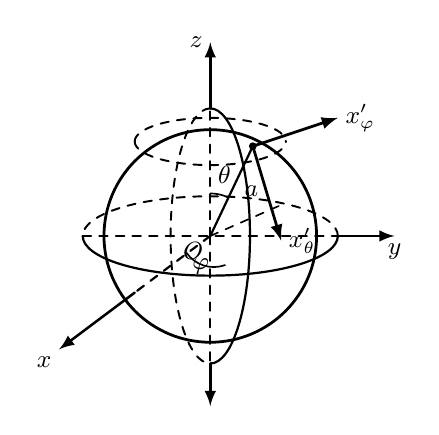
\begin{tikzpicture}[x=1.2cm, y=1.2cm, >=latex, line cap=round, line join=round]
    \draw[line width=1.0pt] (0, 0) circle (1.35cm);

    \draw[line width=0.8pt, dashed] (0, 0) -- (0, 1.35);
    \draw[line width=0.8pt, dashed] (0, 0) -- (0, -1.35);
    \draw[line width=0.9pt, ->] (0, 1.35) -- (0, 2.05) node[left=-1pt] {\small $z$};
    \draw[line width=0.9pt, ->] (0, -1.35) -- (0, -1.8);

    \draw[line width=0.8pt, dashed] (-1.35, 0) -- (1.35, 0);
    \draw[line width=0.9pt, ->] (1.35, 0) -- (1.95, 0) node[below=-1pt] {\small $y$};

    \draw[line width=0.8pt, dashed] (0, 0) -- (-0.8, -0.6);
    \draw[line width=0.9pt, ->] (-0.8, -0.6) -- (-1.6, -1.2) node[below left=-1pt] {\small $x$};
    \node[below left=-1pt] at (0, 0) {\small $O$};

    \draw[line width=0.7pt, dashed] (1.35, 0) arc[start angle=0, end angle=180, x radius=1.35, y radius=0.42];
    \draw[line width=0.8pt] (-1.35, 0) arc[start angle=180, end angle=360, x radius=1.35, y radius=0.42];

    \draw[line width=0.8pt] (0, 1.35) arc[start angle=90, end angle=-90, x radius=0.42, y radius=1.35];
    \draw[line width=0.7pt, dashed] (0, 1.35) arc[start angle=90, end angle=270, x radius=0.42, y radius=1.35];

    \draw[line width=0.7pt, dashed] (-0.8, 1.0) arc[start angle=180, end angle=360, x radius=0.8, y radius=0.25];
    \draw[line width=0.7pt, dashed] (-0.8, 1.0) arc[start angle=180, end angle=0, x radius=0.8, y radius=0.25];

    \coordinate (P) at (0.45, 0.95);
    \fill (P) circle (1.4pt);

    \draw[line width=0.8pt] (0, 0) -- (P) node[midway, right=1pt] {\small $a$};
    \draw[line width=0.6pt] (0, 0.45) arc[start angle=90, end angle=65, radius=0.45];
    \node at (0.15, 0.65) {\small $\theta$};

    \draw[line width=0.6pt, dashed] (0, 0) -- (0.8, 0.35);
    \draw[line width=0.6pt] (-0.25, -0.18) arc[start angle=215, end angle=290, radius=0.35];
    \node at (-0.1, -0.32) {\small $\varphi$};

    \draw[line width=1.0pt, ->] (P) -- ++(0.3, -1.0) node[right=-1pt] {\small $\boldsymbol{x}'_\theta$};
    \draw[line width=1.0pt, ->] (P) -- ++(0.9, 0.3) node[right=-1pt] {\small $\boldsymbol{x}'_\varphi$};
  \end{tikzpicture}
  \caption{}\label{fig:9.1.6}
\end{figure}

细心的读者会注意到 $\boldsymbol{x}'_{\theta} \times \boldsymbol{x}'_{\varphi} = F = 0$ 表明两个坐标切向量 $\boldsymbol{x}'_{\theta}$ 与 $\boldsymbol{x}'_{\varphi}$ 正交, 即 $\theta$ 线与 $\varphi$ 线为正交曲线网(\cref{fig:9.1.6}). \qedhere
\end{solution}

更一般地, 我们来求 $n - 1$ 维球面的单位法向量场.

\begin{example}\label{ex:9.1.11}
已知球心在坐标原点, 半径为 $a$ 的 $n - 1$ 维球面
\[
  S^{n-1}(a) = \left\{(x_{1}, x_{2}, \cdots, x_{n}) \in \mathbb{R}^{n} \mathrel{\Big|} \sum_{i=1}^{n}x_{i}^{2} = a^{2}\right\}, \quad a > 0.
\]
求 $n - 1$ 维球面 $S^{n-1}(a)$ 的单位法向量场、球面坐标及第一基本量.
\end{example}

\begin{solution}[解法 1]
令 $F(x_{1}, x_{2}, \cdots, x_{n}) = \sum_{i=1}^{n} x_{i}^{2} - a^{2}$, 则
\[
  F^{\prime}_{x_{i}} = 2x_{i}.
\]
因此, 单位法向量场为
\begin{align*}
  \boldsymbol{n}_{0} &= \pm\frac{1}{\sqrt{\sum_{i=1}^{n}(F_{x_{i}}^{\prime})^{2}}}(F_{x_{1}}^{\prime}, F_{x_{2}}^{\prime}, \cdots, F_{x_{n}}^{\prime}) = \pm\frac{1}{\sqrt{\sum_{i=1}^{n}(2x_{i})^{2}}}(2x_{1}, 2x_{2}, \cdots, 2x_{n}) \\
  &= \pm\left(\frac{x_{1}}{a}, \frac{x_{2}}{a}, \cdots, \frac{x_{n}}{a}\right).
\end{align*}
\end{solution}

\begin{solution}[解法 2]
设 $\boldsymbol{x}(\theta_{1}, \theta_{2}, \cdots, \theta_{n-1}) = (x_{1}(\theta_{1}, \cdots, \theta_{n-1}), x_{2}(\theta_{1}, \cdots, \theta_{n-1}), \cdots, x_{n}(\theta_{1}, \cdots, \theta_{n-1}))$, 其中
\[
  \left\{\begin{aligned}
    x_{1} &= a\cos\theta_{1}, \\
    x_{2} &= a\sin\theta_{1}\cos\theta_{2}, \\
    x_{3} &= a\sin\theta_{1}\sin\theta_{2}\cos\theta_{3}, \\
    &\;\;\vdots \\
    x_{n-1} &= a\sin\theta_{1}\sin\theta_{2}\sin\theta_{3}\cdots\sin\theta_{n-2}\cos\theta_{n-1}, \\
    x_{n} &= a\sin\theta_{1}\sin\theta_{2}\sin\theta_{3}\cdots\sin\theta_{n-2}\sin\theta_{n-1},
  \end{aligned}\right.
\]
而 $\theta_{1}, \theta_{2}, \cdots, \theta_{n-1}$ 称为球面参数, 也称为球面坐标. 不难验证第一基本量为
\[
  g_{ij} = \boldsymbol{x}^{\prime}_{\theta_{i}} \cdot \boldsymbol{x}^{\prime}_{\theta_{j}} = \left\{\begin{aligned}
    &0, && i \neq j, \\
    &a^{2}, && i = j = 1, \\
    &a^{2}\sin^{2}\theta_{1}\cdots\sin^{2}\theta_{i-1}, && i = j = 2, 3, \cdots, n - 1.
  \end{aligned}\right.
\]
由此得到 $\sqrt{\det(g_{ij})} = a^{n-1}\sin^{n-2}\theta_1\sin^{n-3}\theta_2\cdots\sin\theta_{n-2}$.

对 $\boldsymbol{x} \cdot \boldsymbol{x} = a^{2}$ 两边关于 $\theta_{i}$ 求偏导或直接对 $\boldsymbol{x}$ 关于 $\theta_{i}$ 求偏导验证得 $\boldsymbol{x} \cdot \dfrac{\partial\boldsymbol{x}}{\partial\theta_{i}} = 0$, $i = 1, 2, \cdots, n - 1$ 可知, $\boldsymbol{x}$ 为球面 $M$ 的法向量场. 因此, 单位法向量场为
\[
  \boldsymbol{n}_{0} = \pm\frac{\boldsymbol{x}}{\|\boldsymbol{x}\|} = \pm\frac{\boldsymbol{x}}{a} = \pm\left(\frac{x_{1}}{a}, \frac{x_{2}}{a}, \cdots, \frac{x_{n}}{a}\right). \qedhere
\]
\end{solution}

\begin{example}\label{ex:9.1.12}
{\emergencystretch=3em 从球面坐标, 平面极坐标 $(x_{1}, x_{2}) = (r \cos \theta, r \sin \theta)$ 以及三维 Euclid 空间 $\mathbb{R}^{3}$ 中的球坐标 $(x_{1}, x_{2}, x_{3}) = (r \cos \theta_{1}, r \sin \theta_{1} \cos \theta_{2}, r \sin \theta_{1} \sin \theta_{2})$ 或者 $(r \sin \theta \cos \varphi, r \sin \theta \sin \varphi, r \cos \theta)$(\cref{fig:9.1.7}), 自然会想到 $n$ 维 Euclid 空间 $\mathbb{R}^{n}$ 中应有球坐标.\par}

\begin{figure}[htbp]
  \centering
  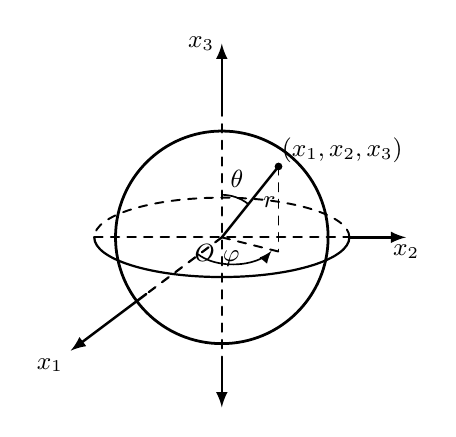
\begin{tikzpicture}[x=1.2cm, y=1.2cm, >=latex, line cap=round, line join=round]
    \draw[line width=1.0pt] (0, 0) circle (1.35cm);

    \draw[line width=0.8pt, dashed] (0, -1.35) -- (0, 1.35);
    \draw[line width=0.9pt, ->] (0, 1.35) -- (0, 2.05) node[left=-1pt] {\small $x_3$};
    \draw[line width=0.9pt, ->] (0, -1.35) -- (0, -1.8);

    \draw[line width=0.8pt, dashed] (-1.35, 0) -- (1.35, 0);
    \draw[line width=0.9pt, ->] (1.35, 0) -- (1.95, 0) node[below=-1pt] {\small $x_2$};

    \draw[line width=0.8pt, dashed] (0, 0) -- (-0.8, -0.6);
    \draw[line width=0.9pt, ->] (-0.8, -0.6) -- (-1.6, -1.2) node[below left=-1pt] {\small $x_1$};
    \node[below left=-1pt] at (0, 0) {\small $O$};

    \draw[line width=0.7pt, dashed] (1.35, 0) arc[start angle=0, end angle=180, x radius=1.35, y radius=0.42];
    \draw[line width=0.8pt] (-1.35, 0) arc[start angle=180, end angle=360, x radius=1.35, y radius=0.42];

    \coordinate (P) at (0.6, 0.75);
    \fill (P) circle (1.4pt) node[anchor=south west, inner sep=1pt] {\small $(x_1, x_2, x_3)$};

    \coordinate (Pxy) at (0.6, -0.15);
    \draw[line width=0.7pt, dashed] (P) -- (Pxy);
    \draw[line width=0.7pt, dashed] (0, 0) -- (Pxy);

    \draw[line width=0.9pt] (0, 0) -- (P) node[midway, right=1pt] {\small $r$};

    \draw[line width=0.6pt] (0, 0.45) arc[start angle=90, end angle=52, radius=0.45];
    \node at (0.16, 0.62) {\small $\theta$};

    \draw[line width=0.6pt, ->] (-0.25, -0.18) arc[start angle=215, end angle=335, x radius=0.45, y radius=0.25];
    \node at (0.1, -0.22) {\small $\varphi$};
  \end{tikzpicture}
  \caption{}\label{fig:9.1.7}
\end{figure}

$\boldsymbol{x}(r, \theta_{1}, \theta_{2}, \cdots, \theta_{n-1}) = (x_{1}(r, \theta_{1}, \cdots, \theta_{n-1}), x_{2}(r, \theta_{1}, \cdots, \theta_{n-1}), \cdots, x_{n}(r, \theta_{1}, \cdots, \theta_{n-1}))$ 为
\[
  \left\{\begin{aligned}
    x_{1} &= r\cos\theta_{1}, \\
    x_{2} &= r\sin\theta_{1}\cos\theta_{2}, \\
    x_{3} &= r\sin\theta_{1}\sin\theta_{2}\cos\theta_{3}, \\
    &\;\;\vdots \\
    x_{n-1} &= r\sin\theta_{1}\sin\theta_{2}\sin\theta_{3}\cdots\sin\theta_{n-2}\cos\theta_{n-1}, \\
    x_{n} &= r\sin\theta_{1}\sin\theta_{2}\sin\theta_{3}\cdots\sin\theta_{n-2}\sin\theta_{n-1},
  \end{aligned}\right.
\]
其中 $r, \theta_{1}, \theta_{2}, \cdots, \theta_{n-1}$ 为 $\mathbb{R}^{n}$ 的参数, 也称为球坐标. 不难验证第一基本量为
\[
  g_{00} = \boldsymbol{x}_{r}^{\prime} \cdot \boldsymbol{x}_{r}^{\prime} = 1,
\]
\[
  g_{0i} = \boldsymbol{x}_{r}^{\prime} \cdot \boldsymbol{x}_{\theta_{i}}^{\prime} = 0 = \boldsymbol{x}_{\theta_{i}}^{\prime} \cdot \boldsymbol{x}_{r}^{\prime} = g_{i0},
\]
\[
  g_{ij} = \left\{\begin{aligned}
    &0, && i \neq j, \\
    &r^{2}, && i = j = 1, \\
    &r^{2}\sin^{2}\theta_{1}\sin^{2}\theta_{2}\cdots\sin^{2}\theta_{i-1}, && i = j = 2, 3, \cdots, n - 1.
  \end{aligned}\right.
\]
由此得到
\begin{align*}
  \left(\frac{\partial(x_{1}, x_{2}, \cdots, x_{n})}{\partial(r, \theta_{1}, \theta_{2}, \cdots, \theta_{n-1})}\right)^{2}
  &= \det\begin{pmatrix}
    \dfrac{\partial x_{1}}{\partial r} & \cdots & \dfrac{\partial x_{n}}{\partial r} \\
    \dfrac{\partial x_{1}}{\partial\theta_{1}} & \cdots & \dfrac{\partial x_{n}}{\partial\theta_{1}} \\
    \vdots & & \vdots \\
    \dfrac{\partial x_{1}}{\partial\theta_{n-1}} & \cdots & \dfrac{\partial x_{n}}{\partial\theta_{n-1}}
  \end{pmatrix}\begin{pmatrix}
    \dfrac{\partial x_{1}}{\partial r} & \dfrac{\partial x_{1}}{\partial\theta_{1}} & \cdots & \dfrac{\partial x_{1}}{\partial\theta_{n-1}} \\
    \vdots & \vdots & & \vdots \\
    \dfrac{\partial x_{n}}{\partial r} & \dfrac{\partial x_{n}}{\partial\theta_{1}} & \cdots & \dfrac{\partial x_{n}}{\partial\theta_{n-1}}
  \end{pmatrix} \\
  &= \det\begin{pmatrix}
    g_{00} & g_{01} & \cdots & g_{0,n-1} \\
    g_{10} & g_{11} & \cdots & g_{1,n-1} \\
    \vdots & \vdots & & \vdots \\
    g_{n-1,0} & g_{n-1,1} & \cdots & g_{n-1,n-1}
  \end{pmatrix} \\
  &= \left[r^{n-1}\sin^{n-2}\theta_{1}\sin^{n-3}\theta_{2}\cdots\sin\theta_{n-2}\right]^{2}.
\end{align*}
如果注意到
\begin{align*}
  \frac{\partial(x_{1}, x_{2}, \cdots, x_{n})}{\partial(r, \theta_{1}, \theta_{2}, \cdots, \theta_{n-1})}\bigg|_{\left(r, \frac{\pi}{2}, \frac{\pi}{2}, \cdots, \frac{\pi}{2}\right)}
  &= \begin{vmatrix}
    0 & -r & 0 & \cdots & 0 \\
    0 & 0 & -r & \cdots & 0 \\
    \vdots & \vdots & \vdots & & \vdots \\
    0 & 0 & 0 & \cdots & -r \\
    1 & 0 & 0 & \cdots & 0
  \end{vmatrix} = (-1)^{1+n}(-r)^{n-1} \\
  &= r^{n-1} > 0,
\end{align*}
及直角坐标 $x_{1}, x_{2}, \cdots, x_{n}$ 与球坐标 $r, \theta_{1}, \theta_{2}, \cdots, \theta_{n-1}$ 之间变换的 Jacobi 行列式
\[
  \frac{\partial(x_{1}, x_{2}, \cdots, x_{n})}{\partial(r, \theta_{1}, \theta_{2}, \cdots, \theta_{n-1})}
\]
为连续函数, 它具有保号性, 因此有
\[
  \frac{\partial(x_{1}, x_{2}, \cdots, x_{n})}{\partial(r, \theta_{1}, \theta_{2}, \cdots, \theta_{n-1})} > 0.
\]
从而
\begin{align*}
  \frac{\partial(x_{1}, x_{2}, \cdots, x_{n})}{\partial(r, \theta_{1}, \theta_{2}, \cdots, \theta_{n-1})}
  &= \sqrt{\det\begin{pmatrix}
    g_{00} & g_{01} & \cdots & g_{0,n-1} \\
    g_{10} & g_{11} & \cdots & g_{1,n-1} \\
    \vdots & \vdots & & \vdots \\
    g_{n-1,0} & g_{n-1,1} & \cdots & g_{n-1,n-1}
  \end{pmatrix}} \\
  &= r^{n-1}\sin^{n-2}\theta_{1}\sin^{n-3}\theta_{2}\cdots\sin\theta_{n-2}.
\end{align*}
此行列式在应用 $n$ 元球坐标变换计算 $n$ 重积分时非常重要与简便.
\end{example}


\begin{example}\label{ex:9.1.13}
设 $U\subsetneq\mathbb{R}^{3}$ 为开集, $F, G\colon U \to \mathbb{R}^{1}$ 为两个三元函数,
\[
  L = \{(x, y, z) \in \mathbb{R}^{3} \mid F(x, y, z) = 0, \; G(x, y, z) = 0\},\quad
  \boldsymbol{x}^{0} = (x_{0}, y_{0}, z_{0}) \in L.
\]
如果 $F, G \in C^{k}(U, \mathbb{R}^{1})$, $k \geqslant 1$, 且 $\boldsymbol{x}^{0}$ 处的切向量
\[
  \boldsymbol{t}(\boldsymbol{x}^{0}) = \boldsymbol{J}\boldsymbol{F}(\boldsymbol{x}^{0}) \times
  \boldsymbol{J}\boldsymbol{G}(\boldsymbol{x}^{0}) =
  \begin{vmatrix}
    \boldsymbol{i} & \boldsymbol{j} & \boldsymbol{k} \\\\
    F_{x}^{\prime} & F_{y}^{\prime} & F_{z}^{\prime} \\\\
    G_{x}^{\prime} & G_{y}^{\prime} & G_{z}^{\prime}
  \end{vmatrix} \neq \boldsymbol{0},
\]
则 $\exists\,\boldsymbol{x}^{0}$ 的开邻域 $U_{0} \subset U$, s.\,t. $U_{0} \cap L$ 为一段 $C^{k}$ 参数曲线. 这时, $L$ 在 $\boldsymbol{x}^{0}$ 处的切线方程为
\[
  \left\{\begin{aligned}
    &F_{x}^{\prime}(\boldsymbol{x}^{0})(x - x_{0}) + F_{y}^{\prime}(\boldsymbol{x}^{0})(y - y_{0}) + F_{z}^{\prime}(\boldsymbol{x}^{0})(z - z_{0}) = 0, \\\\
    &G_{x}^{\prime}(\boldsymbol{x}^{0})(x - x_{0}) + G_{y}^{\prime}(\boldsymbol{x}^{0})(y - y_{0}) + G_{z}^{\prime}(\boldsymbol{x}^{0})(z - z_{0}) = 0.
  \end{aligned}\right.
\]

\begin{proof}
不妨设
\[
  \frac{\partial(F, G)}{\partial(y, z)}\bigg|_{\boldsymbol{x}^{0}} \neq 0.
\]
由隐函数定理, 存在含 $x_{0}$ 的开区间 $I$ 与含 $(y_{0}, z_{0})$ 的开区间 $J$ 使得方程组
\[
  F(x, y, z) = 0, \quad G(x, y, z) = 0
\]
在含 $\boldsymbol{x}^{0}$ 的开邻域 $U_{0} = I \times J$ 内有
\[
  y = f(x), \quad z = g(x), \quad x \in I,
\]
且 $f, g \in C^{k}(I, \mathbb{R}^{1})$. 因此, $U_{0} \cap L$ 为一段 $C^{k}$ 参数曲线
$\boldsymbol{x} = \boldsymbol{x}(x) = (x, f(x), g(x))$, $x$ 为其参数. 该曲线在 $\boldsymbol{x}^{0}$ 处的切向量为 $(1, f^{\prime}(x_{0}), g^{\prime}(x_{0}))$. 又因为
\[
  F(x, f(x), g(x)) \equiv 0, \quad G(x, f(x), g(x)) \equiv 0,
\]
所以
\[
  \left\{\begin{aligned}
    &F_{x}^{\prime} + F_{y}^{\prime}f^{\prime}(x) + F_{z}^{\prime}g^{\prime}(x) = 0, \\\\
    &G_{x}^{\prime} + G_{y}^{\prime}f^{\prime}(x) + G_{z}^{\prime}g^{\prime}(x) = 0,
  \end{aligned}\right.
\]
从而
\begin{align*}
  \bigl(1, f^{\prime}(x_{0}), g^{\prime}(x_{0})\bigr) \parallel \boldsymbol{t}(\boldsymbol{x}^{0})
  &= \bigl(F_{x}^{\prime}(\boldsymbol{x}^{0}), F_{y}^{\prime}(\boldsymbol{x}^{0}), F_{z}^{\prime}(\boldsymbol{x}^{0})\bigr)
     \times \bigl(G_{x}^{\prime}(\boldsymbol{x}^{0}), G_{y}^{\prime}(\boldsymbol{x}^{0}), G_{z}^{\prime}(\boldsymbol{x}^{0})\bigr) \\\\
  &= \boldsymbol{J}\boldsymbol{F}(\boldsymbol{x}^{0}) \times \boldsymbol{J}\boldsymbol{G}(\boldsymbol{x}^{0})
     \ (\text{图} \ \ref{fig:9.1.8}).
\end{align*}
\begin{figure}[htbp]
  \centering
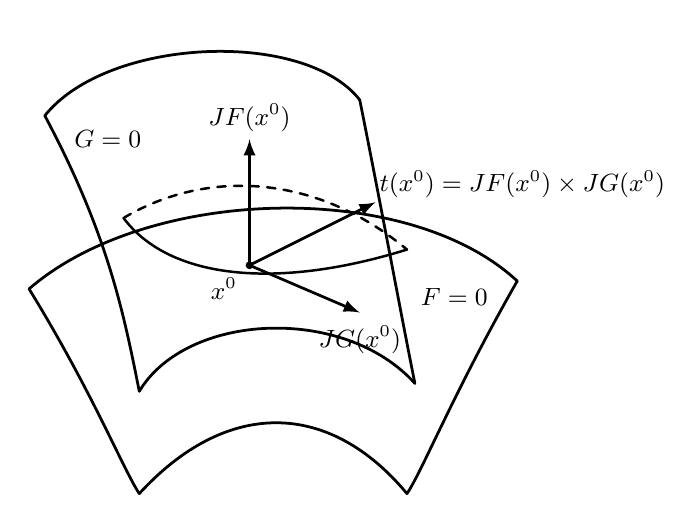
\begin{tikzpicture}[x=1.0cm, y=1.0cm, >=latex, line cap=round, line join=round]
    % 曲面 G=0 (后上)
    \draw[line width=1.0pt] (-2.8, 2.7) .. controls (-2.0, 3.7) and (0.5, 3.8) .. (1.2, 2.9);
    \draw[line width=1.0pt] (-2.8, 2.7) .. controls (-2.0, 1.2) and (-1.8, 0.2) .. (-1.6, -0.8);
    \draw[line width=1.0pt] (1.2, 2.9) .. controls (1.5, 1.4) and (1.7, 0.3) .. (1.9, -0.7);
    \draw[line width=1.0pt] (-1.6, -0.8) .. controls (-1.0, 0.2) and (1.0, 0.3) .. (1.9, -0.7);
    \node at (-2.0, 2.4) {\small $G = 0$};

    % 曲面 F=0 (横跨相交)
    \draw[line width=1.0pt] (-3.0, 0.5) .. controls (-1.5, 1.8) and (1.8, 1.9) .. (3.2, 0.6);
    \draw[line width=1.0pt] (-3.0, 0.5) .. controls (-2.2, -0.8) and (-1.8, -1.8) .. (-1.6, -2.1);
    \draw[line width=1.0pt] (3.2, 0.6) .. controls (2.4, -0.8) and (2.0, -1.8) .. (1.8, -2.1);
    \draw[line width=1.0pt] (-1.6, -2.1) .. controls (-0.5, -0.9) and (0.8, -0.9) .. (1.8, -2.1);
    \node at (2.4, 0.4) {\small $F = 0$};

    % 交线 (鞍形弧线，部分虚线)
    \draw[line width=0.9pt, dashed] (-1.8, 1.4) .. controls (-0.8, 2.0) and (0.6, 2.0) .. (1.8, 1.0);
    \draw[line width=0.9pt] (-1.8, 1.4) .. controls (-1.2, 0.6) and (0.2, 0.5) .. (1.8, 1.0);

    % 相交点 x^0
    \coordinate (X0) at (-0.2, 0.8);
    \fill (X0) circle (1.4pt) node[below left=1pt] {\small $\boldsymbol{x}^0$};

    % 法向量 JF 与 JG
    \draw[line width=1.0pt, ->] (X0) -- ++(0, 1.6) node[above=-1pt] {\small $\boldsymbol{J}F(\boldsymbol{x}^0)$};
    \draw[line width=1.0pt, ->] (X0) -- ++(1.4, -0.6) node[below=1pt] {\small $\boldsymbol{J}G(\boldsymbol{x}^0)$};

    % 切向量 t(x^0) = JF x JG
    \draw[line width=1.0pt, ->] (X0) -- ++(1.6, 0.8) node[anchor=south west, inner sep=1pt] {\small $\boldsymbol{t}(\boldsymbol{x}^0) = \boldsymbol{J}F(\boldsymbol{x}^0) \times \boldsymbol{J}G(\boldsymbol{x}^0)$};
  \end{tikzpicture}
  \caption{}\label{fig:9.1.8}
\end{figure}

由此知, 切线平行于 $\boldsymbol{t}(\boldsymbol{x}^{0})$, 而切线方程为
\[
  \left\{\begin{aligned}
    &F_{x}^{\prime}(\boldsymbol{x}^{0})(x - x_{0}) + F_{y}^{\prime}(\boldsymbol{x}^{0})(y - y_{0}) + F_{z}^{\prime}(\boldsymbol{x}^{0})(z - z_{0}) = 0, \\\\
    &G_{x}^{\prime}(\boldsymbol{x}^{0})(x - x_{0}) + G_{y}^{\prime}(\boldsymbol{x}^{0})(y - y_{0}) + G_{z}^{\prime}(\boldsymbol{x}^{0})(z - z_{0}) = 0.
  \end{aligned}\right.
\]
\qedhere
\end{proof}
\end{example}

\begin{example}\label{ex:9.1.14}
设 $\Delta \subset \mathbb{R}^{2}$ 为开区域, 曲面 $M$ 的参数表示为 $\boldsymbol{x}\colon \Delta \to \mathbb{R}^{3}$, 它是 $C^{1}$ 映射. 而 $(u(t), v(t))$ 对应于 $M$ 上的一条 $C^{1}$ 曲线, 其向量形式为
\[
  \boldsymbol{x} = \boldsymbol{x}(u(t), v(t)),
\]
\[
  \mathrm{d}\boldsymbol{x} = \bigl[\boldsymbol{x}_{u}^{\prime}u^{\prime}(t) + \boldsymbol{x}_{v}^{\prime}v^{\prime}(t)\bigr]\mathrm{d}t
  = \boldsymbol{x}_{u}^{\prime}\mathrm{d}u + \boldsymbol{x}_{v}^{\prime}\mathrm{d}v.
\]
弧元 $\mathrm{d}s$ 的平方为
\begin{align*}
  (\mathrm{d}s)^{2} &= (\mathrm{d}\boldsymbol{x})^{2} = \mathrm{d}\boldsymbol{x}\bullet\mathrm{d}\boldsymbol{x} \\\\
  &= \bigl[E{u^{\prime}}^{2}(t) + 2Fu^{\prime}(t)v^{\prime}(t) + G{v^{\prime}}^{2}(t)\bigr](\mathrm{d}t)^{2} \\\\
  &= E(\mathrm{d}u)^{2} + 2F\mathrm{d}u\mathrm{d}v + G(\mathrm{d}v)^{2}.
\end{align*}
由此得到 $M$ 上从点 $\boldsymbol{x}(u(\alpha), v(\alpha))$ 到 $\boldsymbol{x}(u(\beta), v(\beta))$ 的曲线的弧长为
\[
  s = \int_{\alpha}^{\beta}\sqrt{E\,{u^{\prime}}^{2}(t) + 2Fu^{\prime}(t)v^{\prime}(t) + G\,{v^{\prime}}^{2}(t)}\;\mathrm{d}t.
\]
考虑例 \ref{ex:9.1.10} 中的球面 $M$ 上的两点 $p$ 与 $q$. 不失一般性, 可设 $p$ 与 $q$ 在 $M$ 的同一条经线上. 设这两点的参数分别为 $(\theta_{0}, \varphi_{0})$ 与 $(\theta_{1}, \varphi_{1})$, 其中 $\theta_{1} > \theta_{0}$. 这两点所决定的球面曲线记为 $\Gamma$, 其 $C^{1}$ 参数表示为
\[
  \bigl(\theta(t), \varphi(t)\bigr), \quad t_{0} \leqslant t \leqslant t_{1}.
\]
于是, $\Gamma$ 的弧长为
\begin{align*}
  s(\Gamma) &= \int_{t_{0}}^{t_{1}}\sqrt{a^{2}\bigl[\theta^{\prime}(t)\bigr]^{2} + a^{2}\sin^{2}\theta(t) \cdot \bigl[\varphi^{\prime}(t)\bigr]^{2}}\;\mathrm{d}t \\\\
  &\geqslant a\int_{t_{0}}^{t_{1}}\theta^{\prime}(t)\mathrm{d}\theta
  = a\bigl[\theta(t_{1}) - \theta(t_{0})\bigr].
\end{align*}
式中等号成立等价于 $\varphi^{\prime}(t) = \vec{0}$ 等价于 $\varphi(t) = \varphi_{0}$ (常值). 这时曲线 $\Gamma$ 正是由 $p$ 与 $q$ 两点所决定的大圆弧, 而
$  a\bigl[\theta(t_{1}) - \theta(t_{0})\bigr] = a(\theta_{1} - \theta_{0})$ 恰为这一段大圆弧的弧长.
\end{example}

\begin{definition}\label{def:9.1.4}
设 $s$ 维 $C^{k}\,(k \geqslant 1)$ 正则曲面 $M$ 的参数表示为 $\boldsymbol{x}(u_{1}, u_{2}, \cdots, u_{s})$, 它的第一基本量为
\[
  g_{ij} = \boldsymbol{x}_{u_{i}}^{\prime} \cdot \boldsymbol{x}_{u_{j}}^{\prime}, \quad i, j = 1, 2, \cdots, s.
\]
我们称
\[
  I = \sum_{i, j = 1}^{s}g_{ij}\mathrm{d}u_{i}\mathrm{d}u_{j}
\]
为曲面 $M$ 或 $\boldsymbol{x}(\boldsymbol{u})$ 的第一基本形式. 易见,
\begin{align*}
  (\mathrm{d}\boldsymbol{x})^{2} &= \mathrm{d}\boldsymbol{x}\bullet\mathrm{d}\boldsymbol{x} \\\\
  &= \Bigl(\sum_{i=1}^{s}\boldsymbol{x}_{u_{i}}^{\prime}\mathrm{d}u_{i}\Bigr)
     \bullet \Bigl(\sum_{j=1}^{s}\boldsymbol{x}_{u_{j}}^{\prime}\mathrm{d}u_{j}\Bigr) \\\\
  &= \sum_{i, j = 1}^{s}\boldsymbol{x}_{u_{i}}^{\prime}\bullet\boldsymbol{x}_{u_{j}}^{\prime}\mathrm{d}u_{i}\mathrm{d}u_{j}
  = \sum_{i, j = 1}^{s}g_{ij}\mathrm{d}u_{i}\mathrm{d}u_{j} = I.
\end{align*}
考察 $M$ 上的曲线 $\boldsymbol{u}(t)$ 或 $\boldsymbol{x}(\boldsymbol{u}(t))$, 则弧元 $\mathrm{d}s$ 的平方为
\begin{align*}
  (\mathrm{d}s)^{2} &= (\mathrm{d}\boldsymbol{x})^{2} = \mathrm{d}\boldsymbol{x}\cdot\mathrm{d}\boldsymbol{x} \\\\
  &= \Bigl(\sum_{i=1}^{s}\boldsymbol{x}_{u_{i}}^{\prime}\mathrm{d}u_{i}\Bigr)
     \cdot \Bigl(\sum_{j=1}^{s}\boldsymbol{x}_{u_{j}}^{\prime}\mathrm{d}u_{j}\Bigr) \\\\
  &= \sum_{i, j = 1}^{s}\boldsymbol{x}_{u_{i}}^{\prime}\cdot\boldsymbol{x}_{u_{j}}^{\prime}\mathrm{d}u_{i}\mathrm{d}u_{j}
  = \sum_{i, j = 1}^{s}g_{ij}\mathrm{d}u_{i}\mathrm{d}u_{j},
\end{align*}
其中 $\mathrm{d}u_{i} = \mathrm{d}u_{i}(t) = u_{i}^{\prime}(t)\mathrm{d}t$. 从 $t_{0}$ 到 $t_{1}$ 相应的弧长为
\[
  s\bigg|_{t_{0}}^{t_{1}} = \int_{t_{0}}^{t_{1}}\sqrt{\sum_{i, j = 1}^{s}g_{ij}u_{i}^{\prime}u_{j}^{\prime}}\;\mathrm{d}t.
\]
当 $s = 2$ 时, $g_{11} = E$, $g_{12} = g_{21} = F$, $g_{22} = G$, 由 $\boldsymbol{x}_{u}^{\prime}\mathrm{d}u$ 与 $\boldsymbol{x}_{v}^{\prime}\mathrm{d}v$ 张成的平行四边形的面积
\begin{align*}
  \mathrm{d}\boldsymbol{\sigma} &= \bigl\lVert\boldsymbol{x}_{u}^{\prime}\mathrm{d}u \times \boldsymbol{x}_{v}^{\prime}\mathrm{d}v\bigr\rVert
  = \bigl\lVert\boldsymbol{x}_{u}^{\prime} \times \boldsymbol{x}_{v}^{\prime}\bigr\rVert\mathrm{d}u\mathrm{d}v \\\\
  &= \sqrt{EG - F^{2}}\;\mathrm{d}u\mathrm{d}v
\end{align*}
称为该曲面的面积元, 也称为二维体积元(图 \ref{fig:9.1.9}).

\begin{figure}[htbp]
  \centering
\begin{tikzpicture}[x=1.0cm, y=1.0cm, >=latex, line cap=round, line join=round]
    % 曲面 M
    \draw[line width=1.0pt] (-0.2, 2.0) .. controls (1.0, 2.8) and (3.0, 2.8) .. (4.0, 1.6);
    \draw[line width=1.0pt] (-0.2, 2.0) .. controls (0.6, 1.4) and (1.4, 1.5) .. (2.2, 0.8)
                            .. controls (3.0, 1.1) and (3.6, 1.2) .. (4.0, 1.6);
    \node at (3.8, 1.2) {\small $M$};

    \coordinate (XUV) at (1.5, 1.8);

    % 参数网格虚线
    \draw[line width=0.8pt, dashed] (0.3, 1.4) .. controls (1.0, 2.0) and (1.5, 2.3) .. (3.4, 2.3);
    \draw[line width=0.8pt] (0.8, 2.5) .. controls (1.3, 2.0) and (2.0, 1.5) .. (2.7, 0.8);

    % 切平面 (平行四边形外框)
    \coordinate (TP1) at (0.5, 1.8);
    \coordinate (TP2) at (1.6, 3.2);
    \coordinate (TP3) at (3.5, 2.6);
    \coordinate (TP4) at (2.4, 1.2);
    \draw[line width=0.8pt] (TP1) -- (TP2) -- (TP3) -- (TP4) -- cycle;

    % 微元面积平行四边形 (带阴影)
    \coordinate (DP1) at (XUV);
    \coordinate (DP2) at ($(XUV) + (0.3, 1.1)$);
    \coordinate (DP3) at ($(XUV) + (1.5, 1.15)$);
    \coordinate (DP4) at ($(XUV) + (1.2, 0.05)$);

    \fill[pattern=north east lines, pattern color=black!70] (DP1) -- (DP2) -- (DP3) -- (DP4) -- cycle;
    \draw[line width=0.9pt] (DP1) -- (DP2) -- (DP3) -- (DP4) -- cycle;

    % 微元边向量
    \draw[line width=1.0pt, ->] (DP1) -- (DP4) node[right=-1pt] {\small $\boldsymbol{x}'_u \mathrm{d}u$};
    \draw[line width=1.0pt, ->] (DP1) -- (DP2) node[above=-1pt] {\small $\boldsymbol{x}'_v \mathrm{d}v$};

    \fill (XUV) circle (1.4pt) node[below=2pt] {\small $\boldsymbol{x}(u,v)$};
  \end{tikzpicture}
  \caption{}\label{fig:9.1.9}
\end{figure}

更一般地, 由 $\boldsymbol{x}_{u_{i}}^{\prime}\mathrm{d}u_{i}$, $i = 1, 2, \cdots, s$ 张成的 $s$ 维平行 $2s$ 面体的体积
\[
  \mathrm{d}\sigma = \sqrt{\det(g_{ij})}\;\mathrm{d}u_{1}\mathrm{d}u_{2}\cdots\mathrm{d}u_{s}
\]
称为该 $s$ 维曲面的 $s$ 维体积元.
\end{definition}

\begin{example}\label{ex:9.1.15}
求下列曲面的第一基本形式及体积元:

(1) $\mathbb{R}^{3}$ 中二维曲面 $M$, 参数表示为 $\boldsymbol{x}(x, y) = (x, y, z(x, y))$, $z(x, y)$ 为 $C^{1}$ 函数;

(2) $\mathbb{R}^{3}$ 中二维球面 $S^{2}(a)$, 参数表示为
$\boldsymbol{x}(\theta, \varphi) = (a\sin\theta\cos\varphi, a\sin\theta\sin\varphi, a\cos\theta)$, $a > 0$;

(3) $\mathbb{R}^{n}$ 中 $n-1$ 维球面 $S^{n-1}(a)$, 参数表示 $\boldsymbol{x}(\theta_{1}, \theta_{2}, \cdots, \theta_{n-1})$, 如例 \ref{ex:9.1.11} 所示;

(4) $\mathbb{R}^{n}$ 中 $n$ 维参数曲面 $\boldsymbol{x}(r, \theta_{1}, \theta_{2}, \cdots, \theta_{n-1})$, 如例 \ref{ex:9.1.12} 所示.

\begin{solution}
(1) 因为
\[
  \boldsymbol{x}_{x}^{\prime} = (1, 0, z_{x}^{\prime}), \quad \boldsymbol{x}_{y}^{\prime} = (0, 1, z_{y}^{\prime}),
\]
\[
  \begin{pmatrix} g_{11} & g_{12} \\ g_{21} & g_{22} \end{pmatrix}
  = \begin{pmatrix} E & F \\ F & G \end{pmatrix}
  = \begin{pmatrix} 1 + {z^{\prime}}_{x}^{2} & z_{x}^{\prime}z_{y}^{\prime} \\ z_{x}^{\prime}z_{y}^{\prime} & 1 + {z^{\prime}}_{y}^{2} \end{pmatrix},
\]
所以, 曲面 $M$ 的第一基本形式为
\begin{align*}
  I &= E(\mathrm{d}x)^{2} + 2F\mathrm{d}x\mathrm{d}y + G(\mathrm{d}y)^{2} \\\\
  &= (1 + {z_{x}^{\prime}}^{2})(\mathrm{d}x)^{2} + 2z_{x}^{\prime}z_{y}^{\prime}\mathrm{d}x\mathrm{d}y
     + (1 + {z_{y}^{\prime}}^{2})(\mathrm{d}y)^{2}. \qedhere
\end{align*}
而面积元为
\begin{align*}
  \mathrm{d}\sigma &= \sqrt{EG - F^{2}}\;\mathrm{d}x\mathrm{d}y \\\\
  &= \sqrt{(1 + {z_{x}^{\prime}}^{2})(1 + {z_{y}^{\prime}}^{2}) - (z_{x}^{\prime}z_{y}^{\prime})^{2}}\;\mathrm{d}x\mathrm{d}y \\\\
  &= \sqrt{1 + {z_{x}^{\prime}}^{2} + {z_{y}^{\prime}}^{2}}\;\mathrm{d}x\mathrm{d}y.
\end{align*}

(2) 由例 \ref{ex:9.1.10} 解法 2 知, 二维球面 $M$ 的第一基本形式为
\[
  I = a^{2}(\mathrm{d}\theta)^{2} + a^{2}\sin^{2}\theta(\mathrm{d}\varphi)^{2}.
\]
而面积元为
\[
  \mathrm{d}\sigma = \sqrt{EG - F^{2}}\;\mathrm{d}\theta\mathrm{d}\varphi = a^{2}\sin\theta\;\mathrm{d}\theta\mathrm{d}\varphi.
\]

(3) 由例 \ref{ex:9.1.11} 的解法 2 知, $n-1$ 维球面 $S^{n-1}(a)$ 的第一基本形式为
\begin{align*}
  I &= a^{2}(\mathrm{d}\theta_{1})^{2} + a^{2}\sin^{2}\theta_{1}(\mathrm{d}\theta_{2})^{2} + \cdots
     + a^{2}\sin^{2}\theta_{1}\cdots\sin^{2}\theta_{i-1}(\mathrm{d}\theta_{i})^{2} \\\\
  &\quad + \cdots + a^{2}\sin^{2}\theta_{1}\cdots\sin^{2}\theta_{n-2}(\mathrm{d}\theta_{n-1})^{2}.
\end{align*}
而面积元为
\begin{align*}
  \mathrm{d}\sigma &= \sqrt{\det(g_{ij})}\;\mathrm{d}\theta_{i}\mathrm{d}\theta_{i+1}\cdots\mathrm{d}\theta_{n-1} \\\\
  &= a^{n-1}\sin^{n-2}\theta_{1}\sin^{n-3}\theta_{2}\cdots\sin^{2}\theta_{n-3}\sin\theta_{n-2}
     \;\mathrm{d}\theta_{1}\mathrm{d}\theta_{2}\cdots\mathrm{d}\theta_{n-1}.
\end{align*}

(4) 由例 \ref{ex:9.1.12} 知, $\boldsymbol{x}(r, \theta_{1}, \theta_{2}, \cdots, \theta_{n-1})$ 的第二基本形式为(原文如此)
\begin{align*}
  I &= \mathrm{d}r^{2} + r^{2}(\mathrm{d}\theta_{1})^{2} + r^{2}\sin^{2}\theta_{1}(\mathrm{d}\theta_{2})^{2} + \cdots \\\\
  &\quad + r^{2}\sin^{2}\theta_{1}\cdots\sin^{2}\theta_{i-1}(\mathrm{d}\theta_{i})^{2}
  + \cdots + r^{2}\sin^{2}\theta_{1}\cdots\sin^{2}\theta_{n-2}(\mathrm{d}\theta_{n-1})^{2}.
\end{align*}
而体积元为
\begin{align*}
  \mathrm{d}v &= \sqrt{\det(g_{ij})}\;\mathrm{d}r\mathrm{d}\theta_{1}\mathrm{d}\theta_{2}\cdots\mathrm{d}\theta_{n-1} \\\\
  &= r^{n-1}\sin^{n-2}\theta_{1}\sin^{n-3}\theta_{2}\cdots\sin^{2}\theta_{n-3}\sin\theta_{n-2}
     \;\mathrm{d}r\mathrm{d}\theta_{1}\mathrm{d}\theta_{2}\cdots\mathrm{d}\theta_{n-1}. \qedhere
\end{align*}
\end{solution}
\end{example}

\begin{exblock}{练习题 9.1}
  \item 求下列曲面在指定点处的法向量, 切平面方程与法线方程:

  (1) $x^{2} + y^{2} + z^{2} = 4$, $\boldsymbol{x}^{0} = \left(1, 1, \sqrt{2}\right)$;

  (2) $z = \arctan \dfrac{y}{x}$, $\boldsymbol{x}^{0} = \left(1, 1, \dfrac{\pi}{4}\right)$;

  (3) $3x^{2} + 2y^{2} - 2z - 1 = 0$, $\boldsymbol{x}^{0} = (1, 1, 2)$;

  (4) $z = y + \ln\left(\dfrac{x}{z}\right)$, $\boldsymbol{x}^{0} = (1, 1, 1)$;

  (5) $y - \mathrm{e}^{2x - z} = 0$, $\dot{\boldsymbol{x}}^{0} = (1, 1, 2)$;

  (6) $\dfrac{x^{2}}{a^{2}} + \dfrac{y^{2}}{b^{2}} + \dfrac{z^{2}}{c^{2}} = 1$,
  $\boldsymbol{x}^{0} = \left(\dfrac{a}{\sqrt{3}}, \dfrac{b}{\sqrt{3}}, \dfrac{c}{\sqrt{3}}\right)$.

  \item 求椭球面 $x^{2} + 2y^{2} + 3z^{2} = 21$ 上所有平行于平面 $x + 4y + 6z = 0$ 的切平面.

  \item 求曲面 $x^{2} + y^{2} + z^{2} = x$ 的切平面, 使其垂直于平面 $x - y - z = 2$ 与 $x - y - \dfrac{z}{2} = 2$.

  \item 求两曲面
  \[ F(x, y, z) = 0, \quad G(x, y, z) = 0 \]
  的交线在 $xOy$ 平面上的投影曲线的切线方程, 并给出求切线方程的条件.

  \item 两相交曲面在交点处的法向量所夹的角称为这两曲面在这一点的夹角. 求圆柱面 $x^{2} + y^{2} = a^{2}$ 与曲面 $bz = xy$ 的夹角.

  \item 求椭球面
  \[ \frac{x^{2}}{a^{2}} + \frac{y^{2}}{b^{2}} + \frac{z^{2}}{c^{2}} = 1 \]
  上的点的法向量与 $x$ 轴和 $z$ 轴夹成等角的点的全体.

  \item 定出正数 $\lambda$, 使曲面 $xyz = \lambda$ 与椭球面
  \[ \frac{x^{2}}{a^{2}} + \frac{y^{2}}{b^{2}} + \frac{z^{2}}{c^{2}} = 1 \]
  在某一点相切, 即有共同的切平面.

  \item 证明: 曲面 $z = x\mathrm{e}^{\frac{x}{y}}$ 上所有切平面都通过原点.

  \item 证明: 曲面 $\sqrt{x} + \sqrt{y} + \sqrt{z} = \sqrt{a}\,(a > 0)$ 的切平面在各坐标平面上割下的诸线段之和为常数.

  \item 证明: 曲面 $F(x - az, y - bz) = 0$ 的所有切平面与某一直线平行, 其中 $a$, $b$ 为常数. 并说明论述中需加什么条件.

  \item 证明: 曲面 $F\left(\dfrac{x-a}{z-c}, \dfrac{y-b}{z-c}\right) = 0$ 的切平面通过一个固定点, 其中 $a$, $b$, $c$ 为常数. 并说明论述中需加什么条件.

  \item 证明: 曲面 $ax + by + cz = \Phi(x^{2} + y^{2} + z^{2})$ 在点 $\boldsymbol{x}^{0} = (x_{0}, y_{0}, z_{0})$ 处的法向量与向量 $(x_{0}, y_{0}, z_{0})$ 和 $(a, b, c)$ 共面. 并说明论述中需加什么条件.

  \item 求下列曲面的 $E$, $F$ 与 $G$, 第一基本形式及面积元:

  (1) 椭球面 $\boldsymbol{x}(u, v) = (a\sin u\cos v, b\sin u\sin v, c\cos u)$;

  (2) 单叶双曲面 $\boldsymbol{x}(u, v) = (a\,\mathrm{ch}\,u\cos v, b\,\mathrm{ch}\,u\sin v, c\,\mathrm{sh}\,u)$;

  (3) 椭圆抛物面 $\boldsymbol{x}(u, v) = \left(u, v, \dfrac{1}{2}\left(\dfrac{u^{2}}{a^{2}} + \dfrac{v^{2}}{b^{2}}\right)\right)$;

  (4) 双曲抛物面 $\boldsymbol{x}(u, v) = (a(u + v), b(u - v), 2uv)$;

  (5) 劈锥面 $\boldsymbol{x}(u, v) = (u\cos v, u\sin v, \varphi(v))$;

  (6) 一般螺面 $\boldsymbol{x}(u, v) = (u\cos v, u\sin v, \varphi(u) + av)$.

  \item 求 $\mathbb{R}^{3}$ 中圆柱面 $\boldsymbol{x}(\theta, z) = (a\cos\theta, a\sin\theta, z)$ 的第一基本形式与面积元.

  \item 设曲面 $M$ 的第一基本形式为
  \[ I = \mathrm{d}u^{2} + (u^{2} + a^{2})\mathrm{d}v^{2}, \]
  求曲面上的曲线 $u = v$ 从 $v_{1}$ 到 $v_{2}\,(> v_{1})$ 这一段的弧长.

  \item 求平面曲线(星形线) $x^{\frac{2}{3}} + y^{\frac{2}{3}} = a^{\frac{2}{3}}\,(a > 0)$ 上任一点处的切线方程, 并证明这些切线被坐标轴所截取的线段等长(应用 $F(x, y) = x^{\frac{2}{3}} + y^{\frac{2}{3}} - a^{\frac{2}{3}} = 0$ 与参数表示 $(x, y) = (a\cos^{3}t, a\sin^{3}t)$ 两种方法求曲线的切向量).

  \item 求下列曲线所示点处的切线与法平面:

  (1) $(x, y, z) = (a\sin^{2}t, b\sin t\cos t, c\cos^{2}t)$, 在点 $t = \dfrac{\pi}{4}$;

  (2) $2x^{2} + 3y^{2} + z^{2} = 9$, $z^{2} = 3x^{2} + y^{2}$, 在点 $(1, -1, -2)$.

  \item 证明: 球面 $x^{2} + y^{2} + z^{2} = \rho^{2}$ 与锥面 $x^{2} + y^{2} = z^{2}\tan^{2}\varphi$ 是正交的($\rho > 0$ 与 $\varphi$ 为常数).

  \item 在曲线 $(x, y, z) = (t, t^{2}, t^{3})$ 上求出一点, 使曲线在此点的切线平行于平面 $x + 2y + z = 4$.

  \item 求函数
  \[ u = \frac{x}{\sqrt{x^{2} + y^{2} + z^{2}}} \]
  沿曲线 $(x, y, z) = (t, 2t^{2}, -2t^{4})$ 在点 $(1, 2, -2)$ 处切线方向的方向导数.

  \item {\emergencystretch=3em 设 $(x_{0}, y_{0}, z_{0})$ 为曲面 $F(x, y, z) = 1$ 的非奇异点(若
  $\bigl(F_{x}^{\prime}(x_{0}, y_{0}, z_{0}),\allowbreak F_{y}^{\prime}(x_{0}, y_{0}, z_{0}),\allowbreak F_{z}^{\prime}(x_{0}, y_{0}, z_{0})\bigr) \neq (0, 0, 0)$, 则称 $(x_{0}, y_{0}, z_{0})$ 为非奇异点; 否则 $(x_{0}, y_{0}, z_{0})$ 称为奇异点), $F$ 在 $(x_{0}, y_{0}, z_{0})$ 的开邻域 $U$ 内可微, 且为 $n$ 次齐次函数. 证明: 曲面在 $(x_{0}, y_{0}, z_{0})$ 处的切平面方程为\par}
  \[
    xF_{x}^{\prime}(x_{0}, y_{0}, z_{0}) + yF_{y}^{\prime}(x_{0}, y_{0}, z_{0})
    + zF_{z}^{\prime}(x_{0}, y_{0}, z_{0}) = n.
  \]

  \item 设 $F(u, v)$ 为 $C^{1}$ 函数, 证明: 曲面 $F(nx - lz, ny - mz) = 0$ 上任一点的切平面都平行于直线 $L\colon \dfrac{x}{l} = \dfrac{y}{m} = \dfrac{z}{n}$.

  \item 从原点向单叶双曲面
  \[ \frac{x^{2}}{a^{2}} + \frac{y^{2}}{b^{2}} - \frac{z^{2}}{c^{2}} = 1 \]
  的切平面引垂线, 求垂足的轨迹.

  \item 设 $a > 0$, $b > 0$, $c > 0$. 证明: $\mathbb{R}^{3}$ 中任意一点 $(x, y, z)$ 处, 有三个彼此正交的二次曲面
  \[ \frac{x^{2}}{a^{2} - \lambda_{i}^{2}} + \frac{y^{2}}{b^{2} - \lambda_{i}^{2}} + \frac{z^{2}}{c^{2} - \lambda_{i}^{2}} = -1, \quad i = 1, 2, 3, \]
  其中 $\lambda_{1}, \lambda_{2}, \lambda_{3}$ 为三个彼此不同的实数.
\end{exblock}

